% Template:     Informe LaTeX
% Documento:    Archivo principal
% Versión:      8.2.6 (06/07/2023)
% Codificación: UTF-8
%
% Autor: Pablo Pizarro R.
%        pablo@ppizarror.com
%
% Manual template: [https://latex.ppizarror.com/informe]
% Licencia MIT:    [https://opensource.org/licenses/MIT]

% CREACIÓN DEL DOCUMENTO
\documentclass[
	spanish, % Idioma: spanish, english, etc.
	letterpaper, oneside
]{article}

% INFORMACIÓN DEL DOCUMENTO
\def\documenttitle {Informe Práctica Profesional II}
\def\documentsubtitle {}
\def\documentsubject {Análisis de datos de la actividad neuronal del ganglio pedal de \textit{Aplysia} en animales jóvenes y viejos}

\def\documentauthor {Nombre del autor}
\def\coursename {Práctica Profesional II}
\def\coursecode {BT5912}

\def\universityname {Universidad de Chile}
\def\universityfaculty {Facultad de Ciencias Físicas y Matemáticas}
\def\universitydepartment {Departamento de Ingeniería Química, Biotecnología y Materiales}
\def\universitydepartmentimage {departamentos/fcfm2}
\def\universitydepartmentimagecfg {height=1.8cm}
\def\universitylocation {Santiago de Chile}

% INTEGRANTES, PROFESORES Y FECHAS
\def\authortable {
	\begin{tabular}{ll}
		Estudiante:
		& \begin{tabular}[t]{l}
                Javiera Rojas M.
		\end{tabular} \\
		
		Supervisora:
		& \begin{tabular}[t]{l}
		Andrea Colins
		\end{tabular} \\
		
		Profesora:
		& \begin{tabular}[t]{l}
		Oriana Salazar A.
		\end{tabular} \\
		
		Auxiliar:
		& \begin{tabular}[t]{l}
		Florencia Ibáñez
		\end{tabular} \\
		
		Empresa:
		& \begin{tabular}[t]{l}
		Universidad de Chile - Facultad de Medicina
		\end{tabular} \\
		
		Dirección Empresa:
		& \begin{tabular}[t]{l}
		Av. Independencia 1027, Independencia, Región Metropolitana
		\end{tabular} \\
		
		Fecha de entrega:
		& \begin{tabular}[t]{l}
		07 / Abril / 2025
		\end{tabular} \\
	\end{tabular}
}

% IMPORTACIÓN DEL TEMPLATE
\input{template}

% INICIO DE PÁGINAS
\begin{document}

% PORTADA
\templatePortrait

% CONFIGURACIÓN DE PÁGINA Y ENCABEZADOS
\templatePagecfg

% RESUMEN O ABSTRACT
\section*{Resumen}

En el siguiente reporte se presenta el trabajo realizado durante la práctica profesional II bajo la supervisión de la Dra. Andrea Colins, cuyo objetivo es analizar datos de la actividad neuronal del ganglio pedal de \textit{Aplysia} en un conjunto de animales jóvenes y viejos, además de aplicar métodos estadísticos para comparar la actividad neuronal entre ambos grupos.\\

Durante el desarrollo de la práctica se logra comprender el ritmo del trabajo de investigación en la universidad, la importancia de la organización, honestidad en los resultados y buenas prácticas de programación \\

Como resultado, se logra un acercamiento al trabajo de investigación de ingeniero en biotecnología en una universidad y 

. Finalmente, luego de aprender el proceso, se detectan limitaciones y se proponen recomendaciones, tales como sugerir una forma distinta de organización de muestras para evitar su acumulación.






% TABLA DE CONTENIDOS - ÍNDICE
\templateIndex

% CONFIGURACIONES FINALES
\templateFinalcfg

% ======================= INICIO DEL DOCUMENTO =======================

%% Template:     Informe LaTeX
% Documento:    Archivo de ejemplo
% Versión:      8.2.6 (06/07/2023)
% Codificación: UTF-8
%
% Autor: Pablo Pizarro R.
%        pablo@ppizarror.com
%
% Manual template: [https://latex.ppizarror.com/informe]
% Licencia MIT:    [https://opensource.org/licenses/MIT]

% ------------------------------------------------------------------------------
% NUEVA SECCIÓN
% ------------------------------------------------------------------------------


En el siguiente reporte se presenta el trabajo realizado durante la práctica profesional II bajo la supervisión de la Dra. Andrea Colins, cuyo objetivo es analizar datos de la actividad neuronal del ganglio pedal de \textit{Aplysia} en un conjunto de animales jóvenes y viejos, además de aplicar métodos estadísticos para comparar la actividad neuronal entre ambos grupos.\\

 Para ello, se inicia con una búsqueda bibliográfica sobre estudios similares tanto en mamíferos como en \textit{Aplysia}, de la cual se identifican experimentos similares en ratas, donde las principales conclusiones indican que, con la edad, ocurre una pérdida de densidad sináptica \cite{bib perdida sinaptica}, un aumento de la cantidad de neuronas con patrones de disparo tipo burst \cite{bib burst}, un aumento de la conductancia de calcio en canales dependientes de voltaje \cite{bib Ca}, facilitando la generación de spikes y, finalmente, una reducción en la conductancia de potasio en canales dependientes de voltaje \cite{bib Potasio}, lo que prolonga la duración del spike.

Por otra parte, en \textit{Aplysia} se ha observado una relación entre el envejecimiento conductual y la disminución de la excitabilidad en las neuronas sensoriales \cite{bib sensoriales}, además de una reducción en la cantidad de spikes y un aumento en su duración sin cambio en el intervalo existente entre spikes \cite{bib cantidad}.

Por otra parte, en \textit{Aplysia} se tiene que existe una relación entre el envejecimiento conductual y la disminución de la excitabilidad en las neuronas sensoriales \cite{bib sensoriales} y que disminuye la cantidad de spikes y aumenta su duración; sin embargo, no varía el intervalo entre spikes \cite{bib cantidad}. \\

Se propone iniciar con un análisis estadístico estándar, donde se reduce el tiempo de grabación a un máximo de 90 segundos tras la aplicación del estímulo y se grafica, por conjunto, el total de neuronas, los Raster plot correspondientes y el promedio global de spikes por tiempo y por neurona.\\

Luego, para clasificar las neuronas según su patrón de disparo, se propone como metodología realizar un análisis similar al propuesto en el paper \textit{``Modular Deconstruction Reveals the Dynamical and Physical Building Blocks of a Locomotion Motor Program''} \cite{AMB}, publicado en 2015. La clasificación se basa en la correlación cruzada de los spikes train discretizados junto con una prueba de permutación en donde se utiliza un intervalo (bin) de un segundo y un desfase máximo (lag máximo) de 20 segundos. \\

Con las neuronas clasificadas según su tipo de disparo, se analiza la cantidad de neuronas de cada tipo utilizando un gráfico circular. Además, se grafica la matriz de similitud del coseno antes y después de la clasificación para comprobar el éxito del agrupamiento. Posteriormente, se generan nuevamente los raster plots, esta vez con las neuronas agrupadas por tipo, y finalmente, se realiza un gráfico de posición donde cada tipo de neurona se representa con un color diferente.\\

De la metodología anterior, se obtienen los siguientes resultados.\\

\begin{figure}
    \centering
    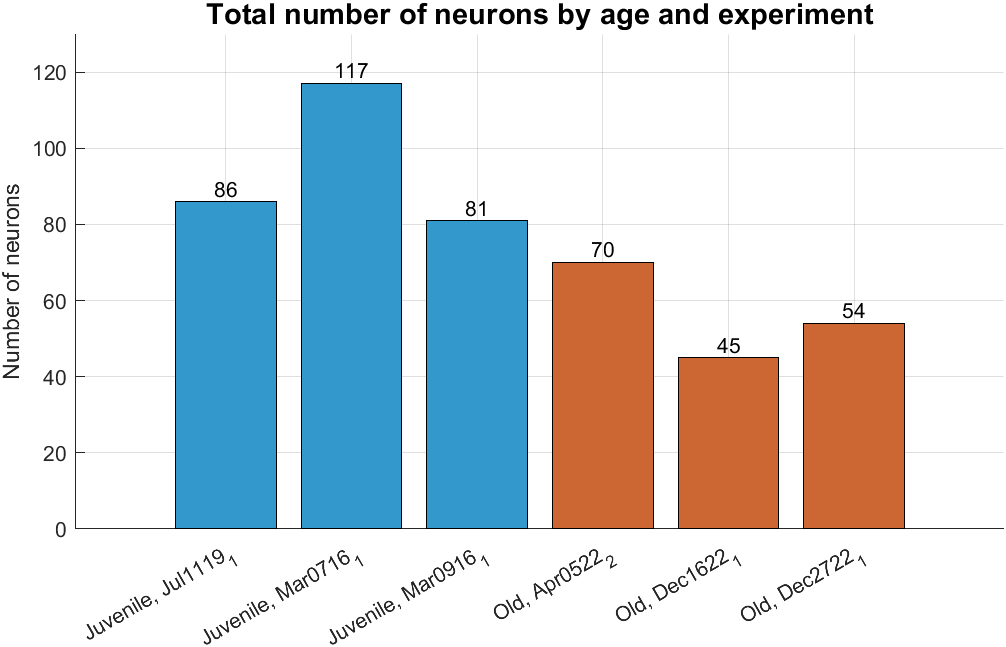
\includegraphics[width=0.8\textwidth]{img/Total_Neurons.png}
    \caption{Total de neuronas por set de datos.}
    \label{total_neurons}
\end{figure}

\begin{figure}
    \centering
    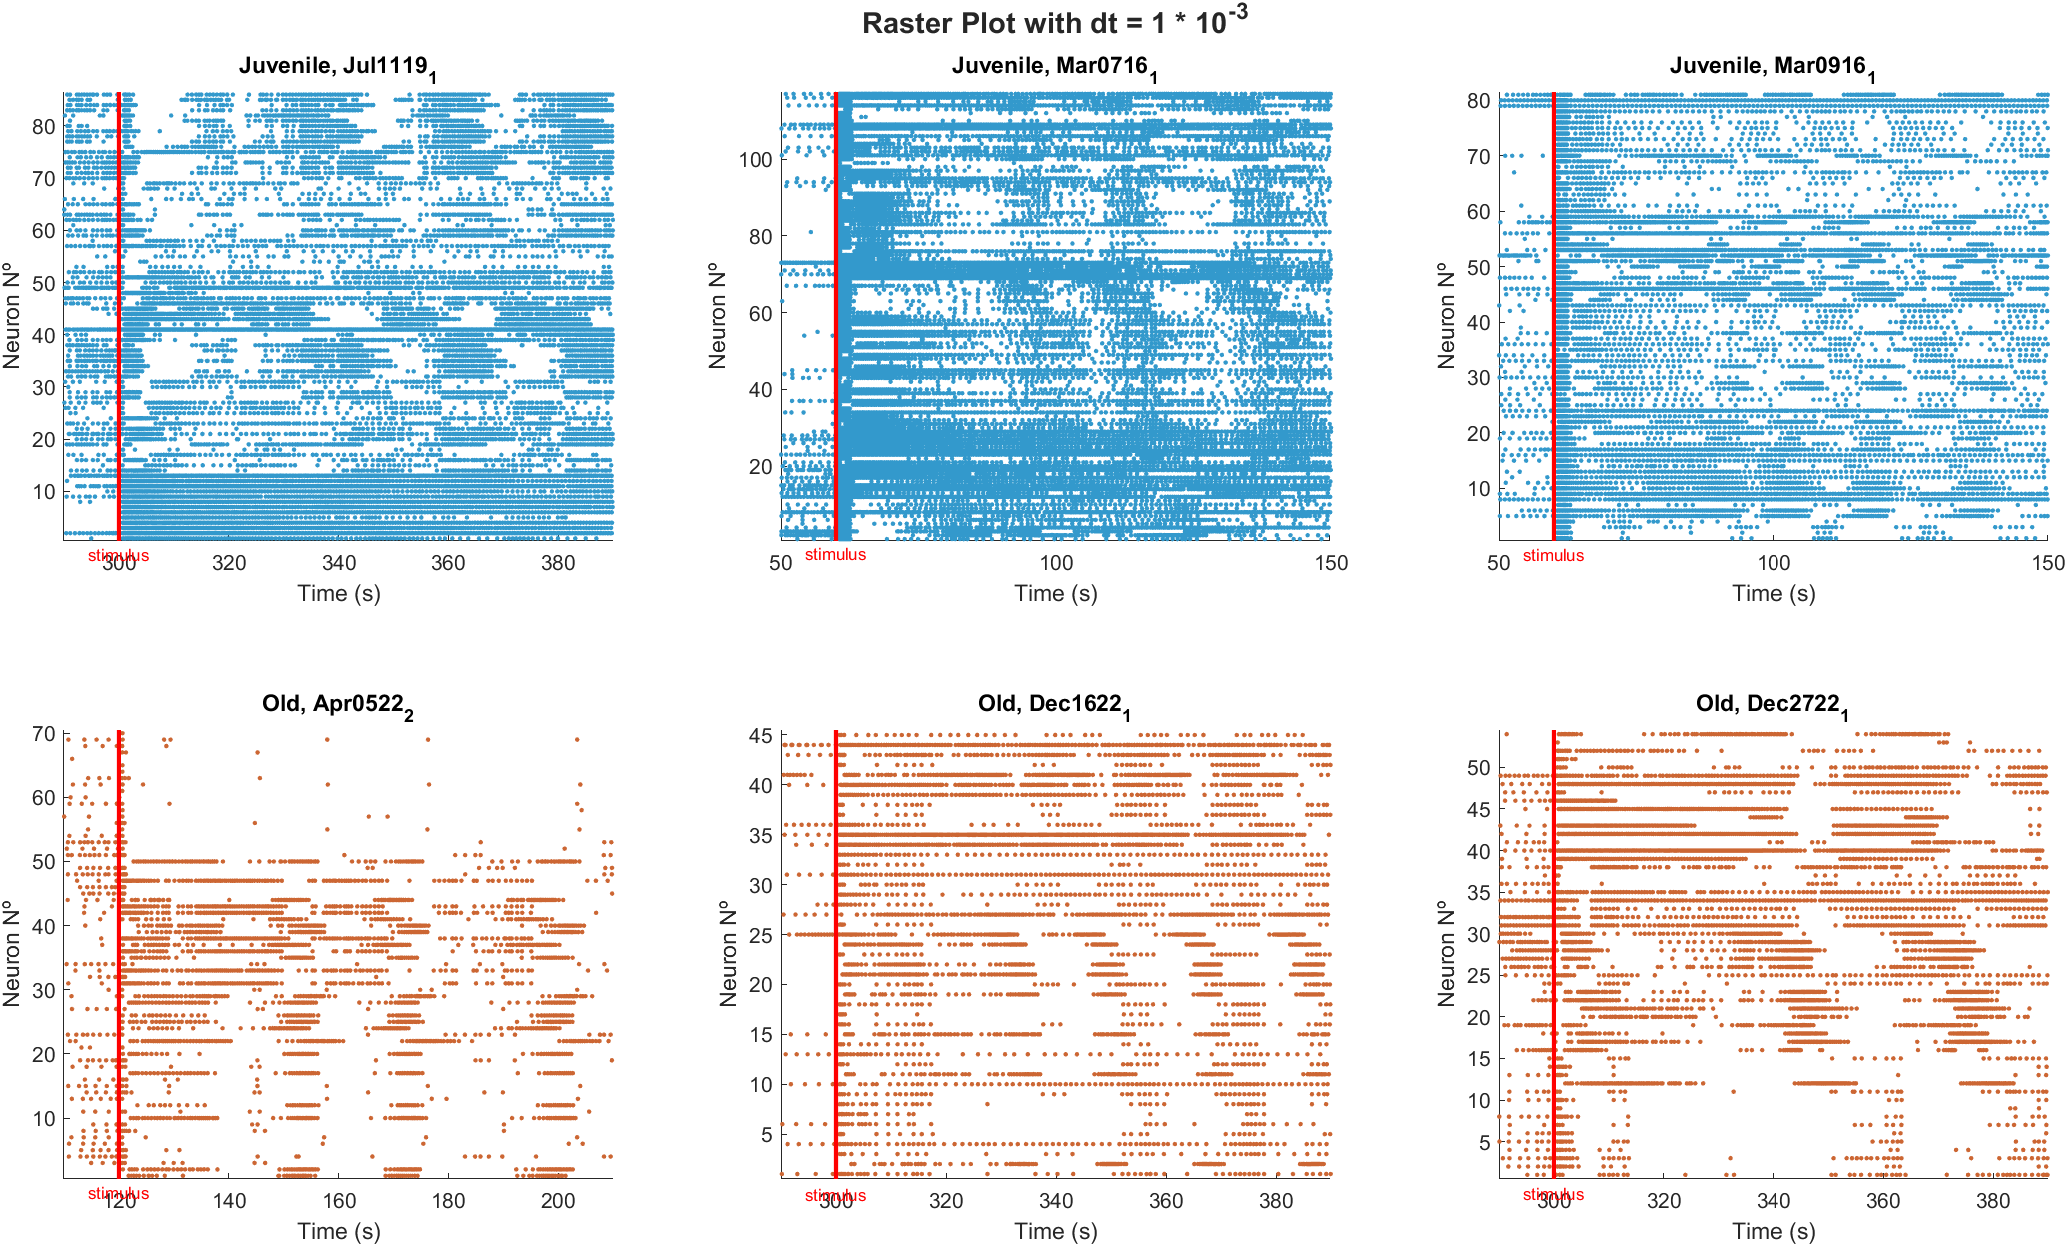
\includegraphics[width=0.9\textwidth]{img/RasterPlot.png}
    \caption{Raster Plot por set de datos.}    
    \label{rasterplot}
\end{figure}

\begin{figure}
    \centering
    \subfloat{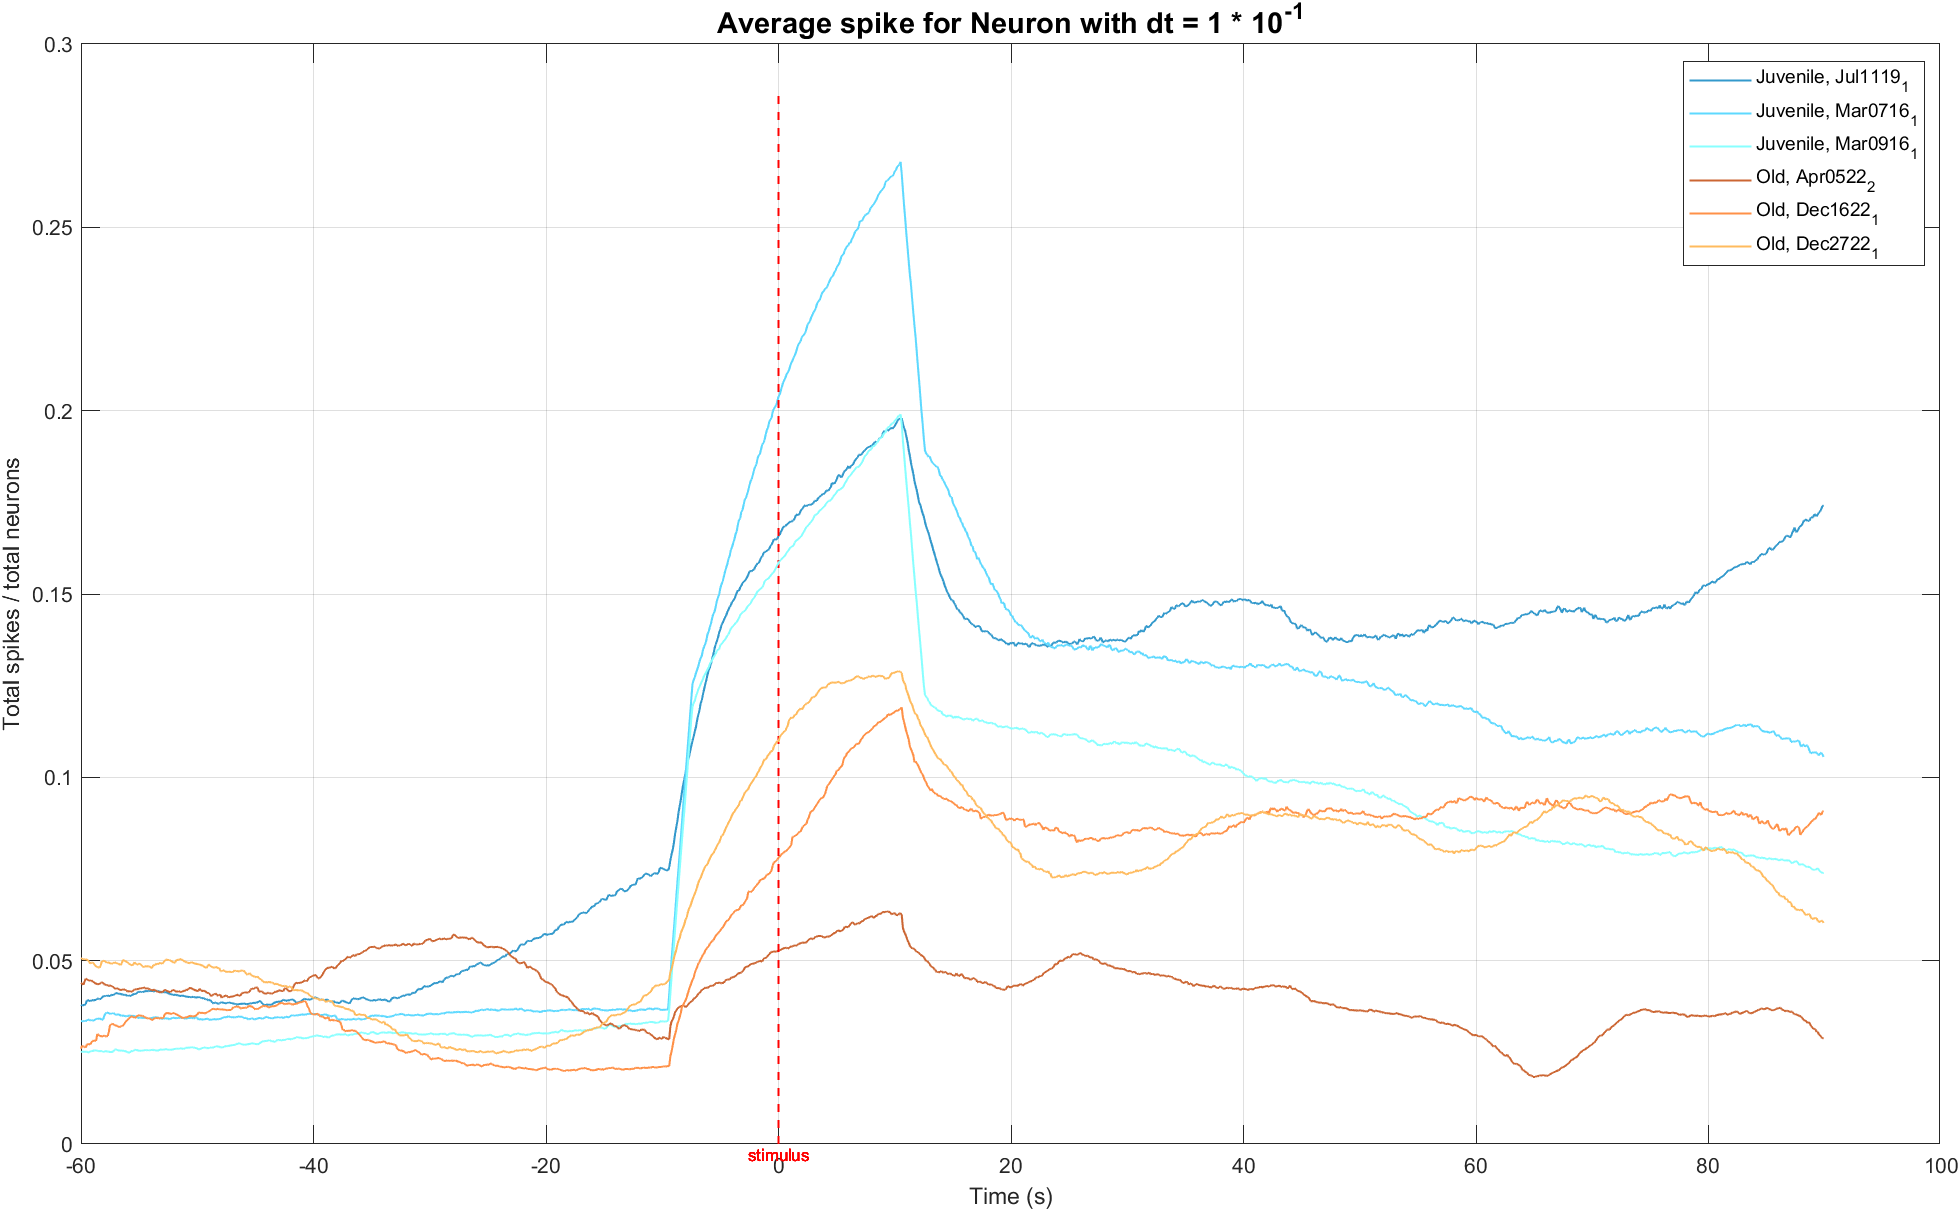
\includegraphics[width=0.8\textwidth]{img/Average_spike_for_Neuron.png}}
    
    \hfill
    
    \subfloat{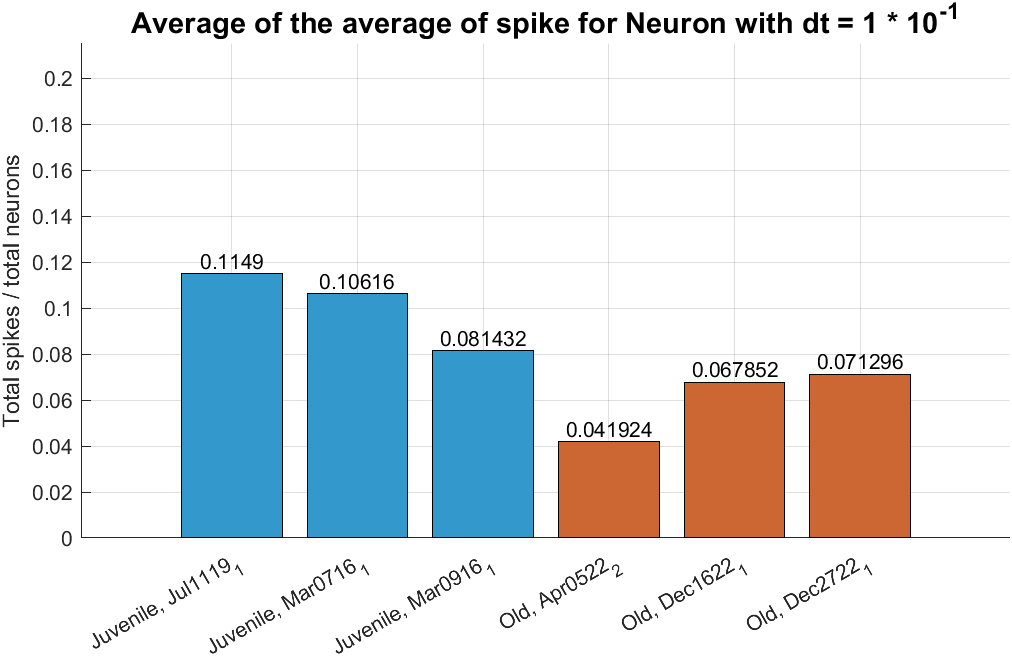
\includegraphics[width=0.8\textwidth]{img/Average_of_the_average_spike_for_Neuron.png}}
    
    \caption{Promedio de spikes totales normalizado por cantidad total de neuronas por set de datos.}
    
    \label{promdelprom}
\end{figure}

\begin{figure}
    \centering
    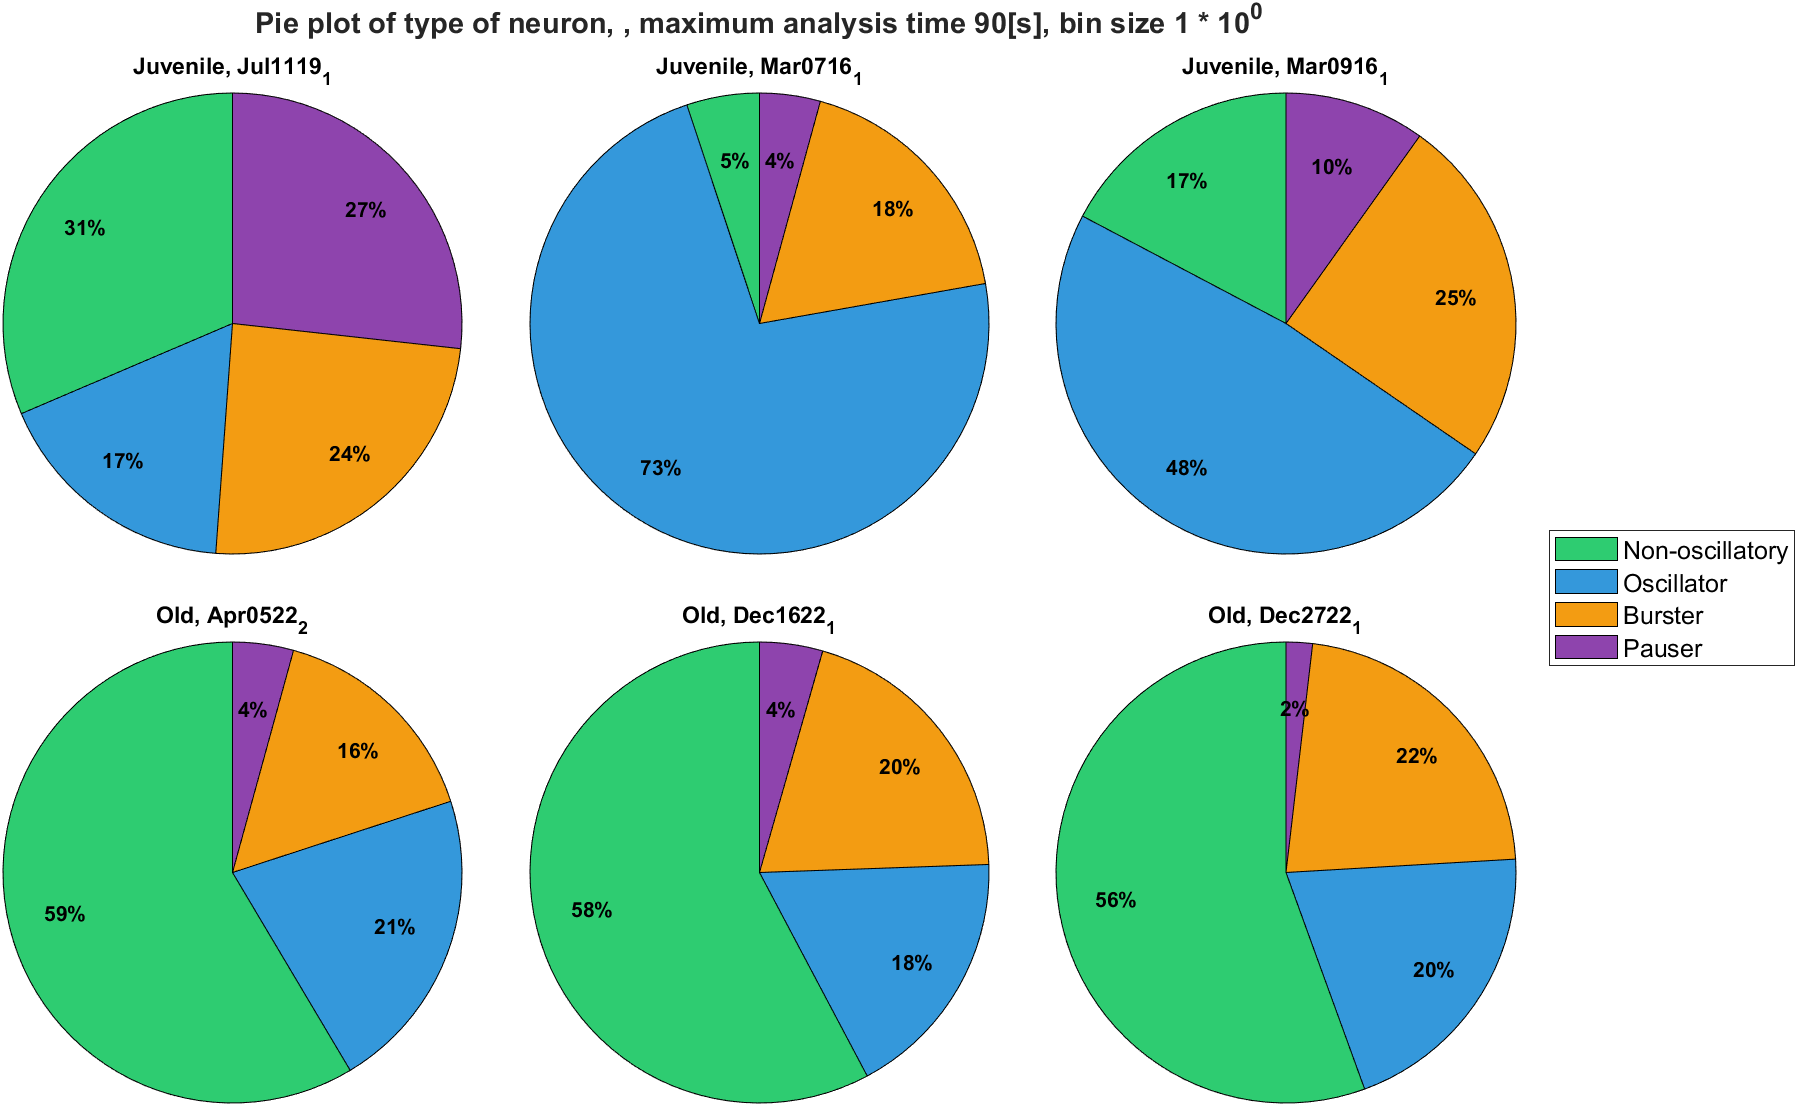
\includegraphics[width=0.8\textwidth]{img/Pie_plot_of_type_of_Neuron.png}
    \caption{Gráfico circular de total de neuronas de cada tipo por set de datos.}    
    \label{pieplot}
\end{figure}

\begin{figure}
    \centering
    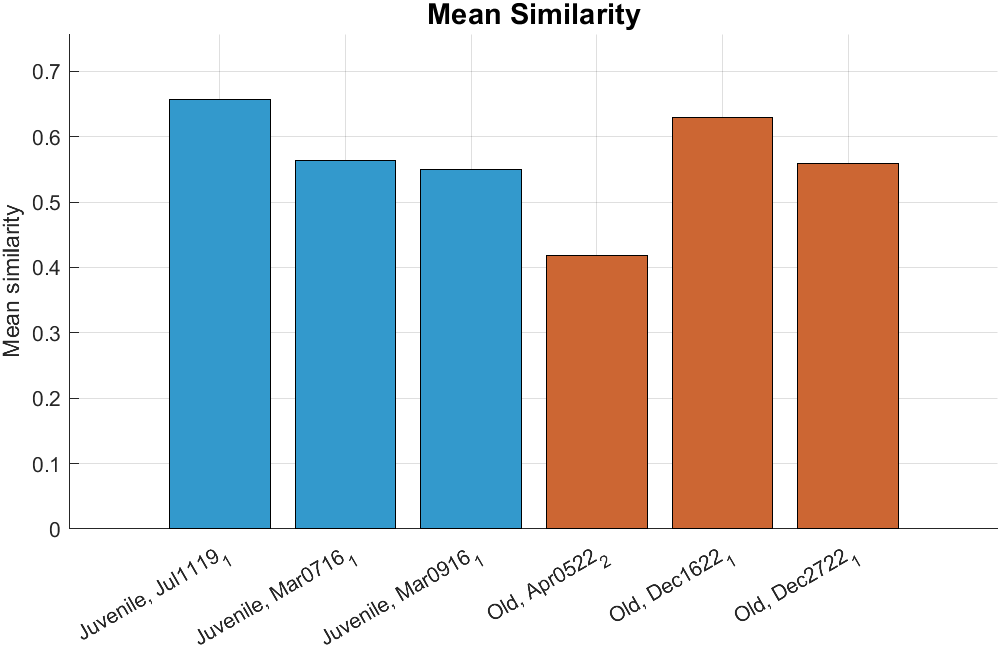
\includegraphics[width=0.8\textwidth]{img/Mean_similarity.png}
    \caption{Promedio de similaridad en matrix de similaridad del coseno por set de datos.}    
    \label{pieplot}
\end{figure}


\begin{figure}
    \centering
    \subfloat{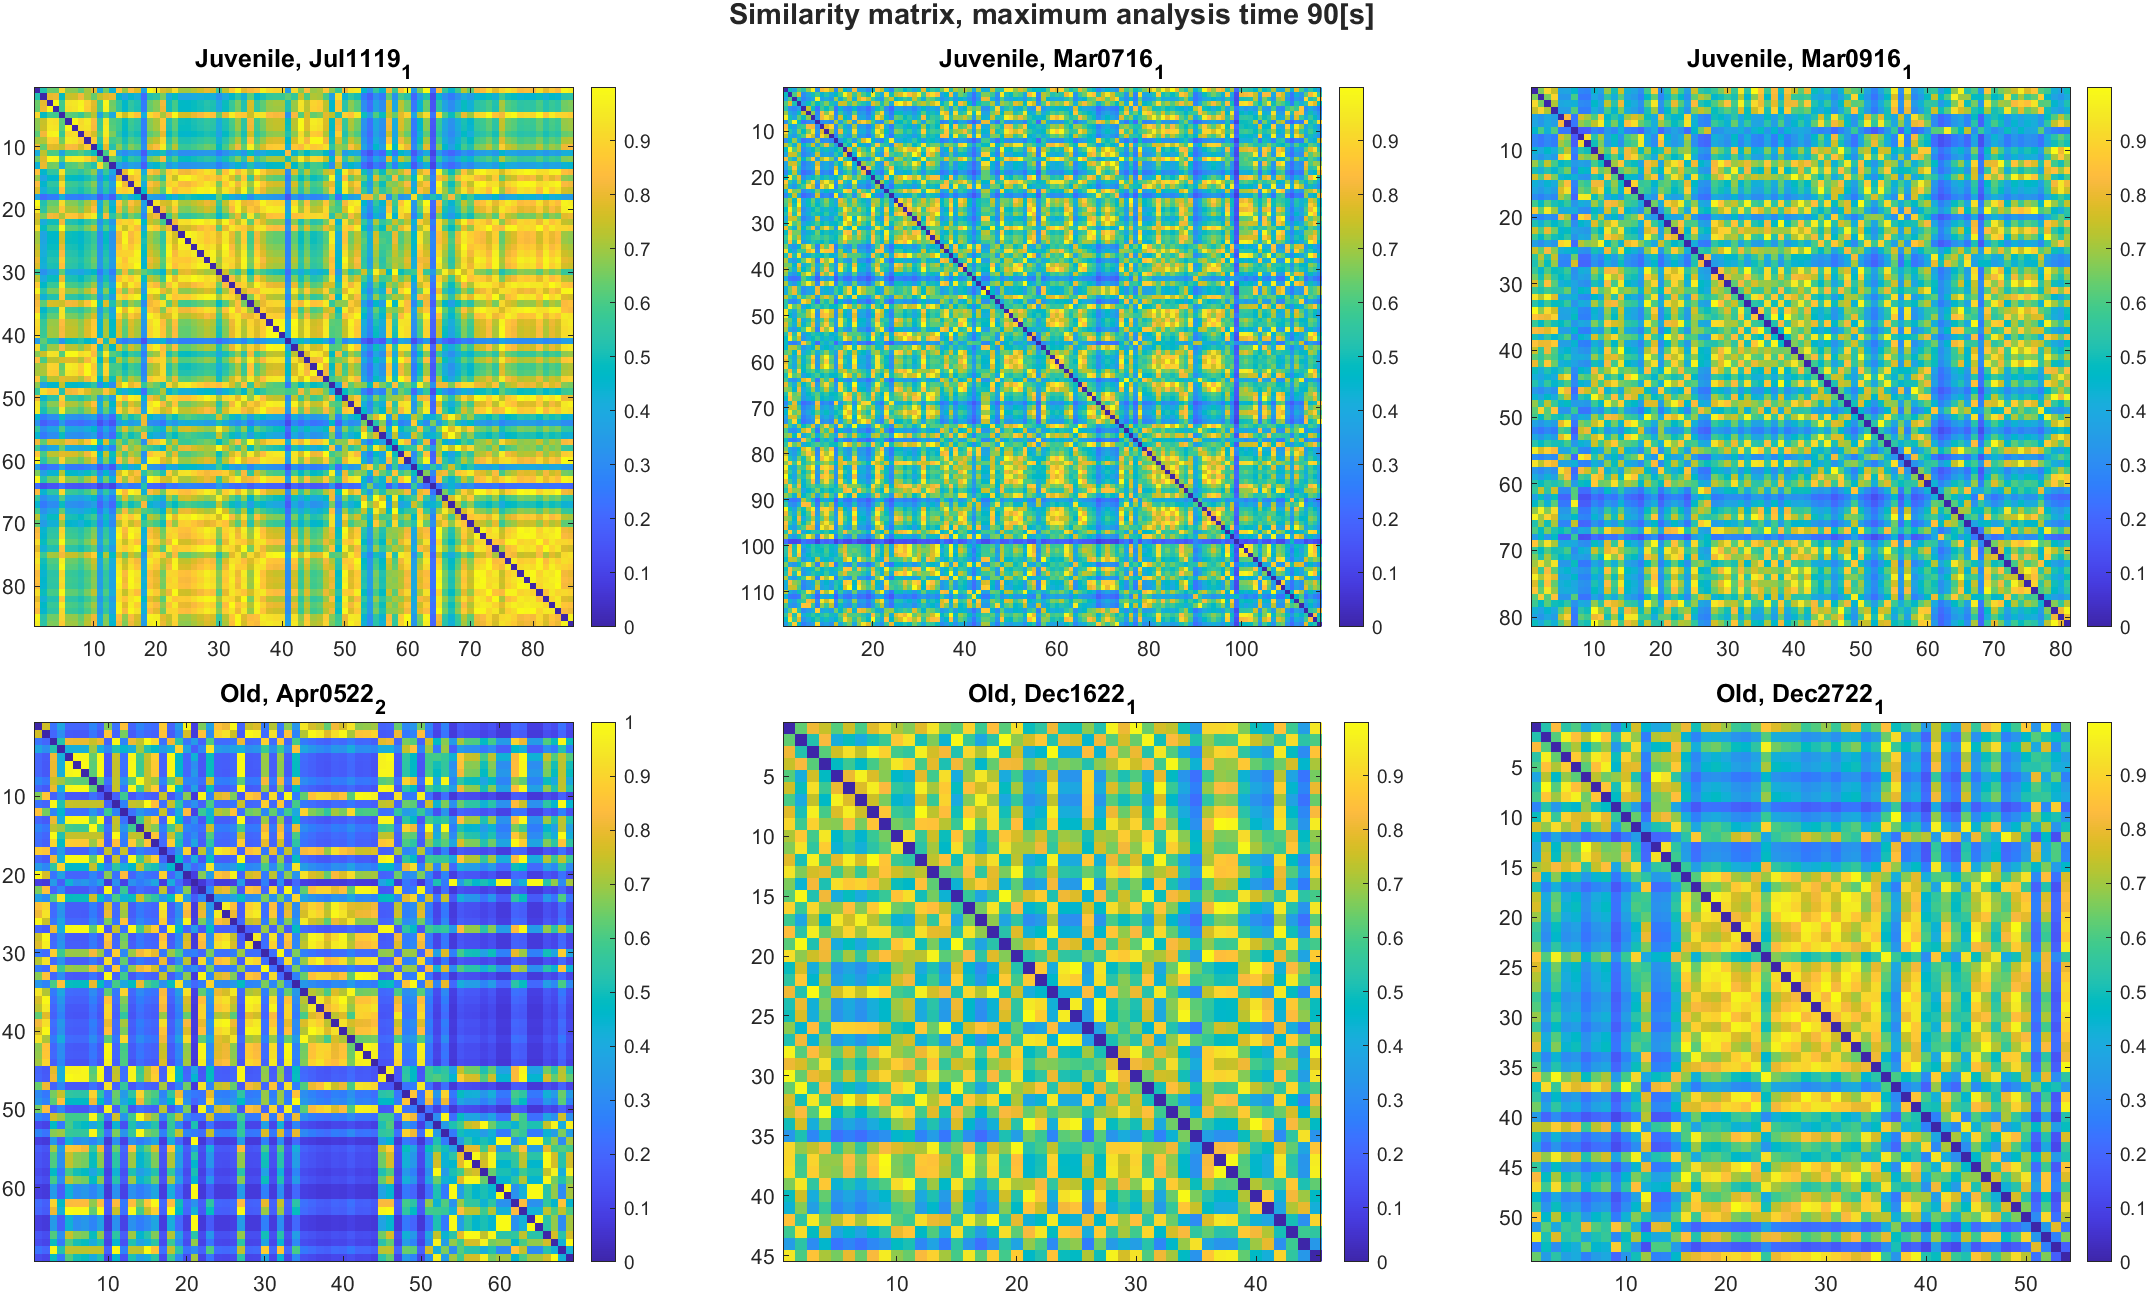
\includegraphics[width=0.8\textwidth]{img/CSM_base.png}}
    
    \hfill
    
    \subfloat{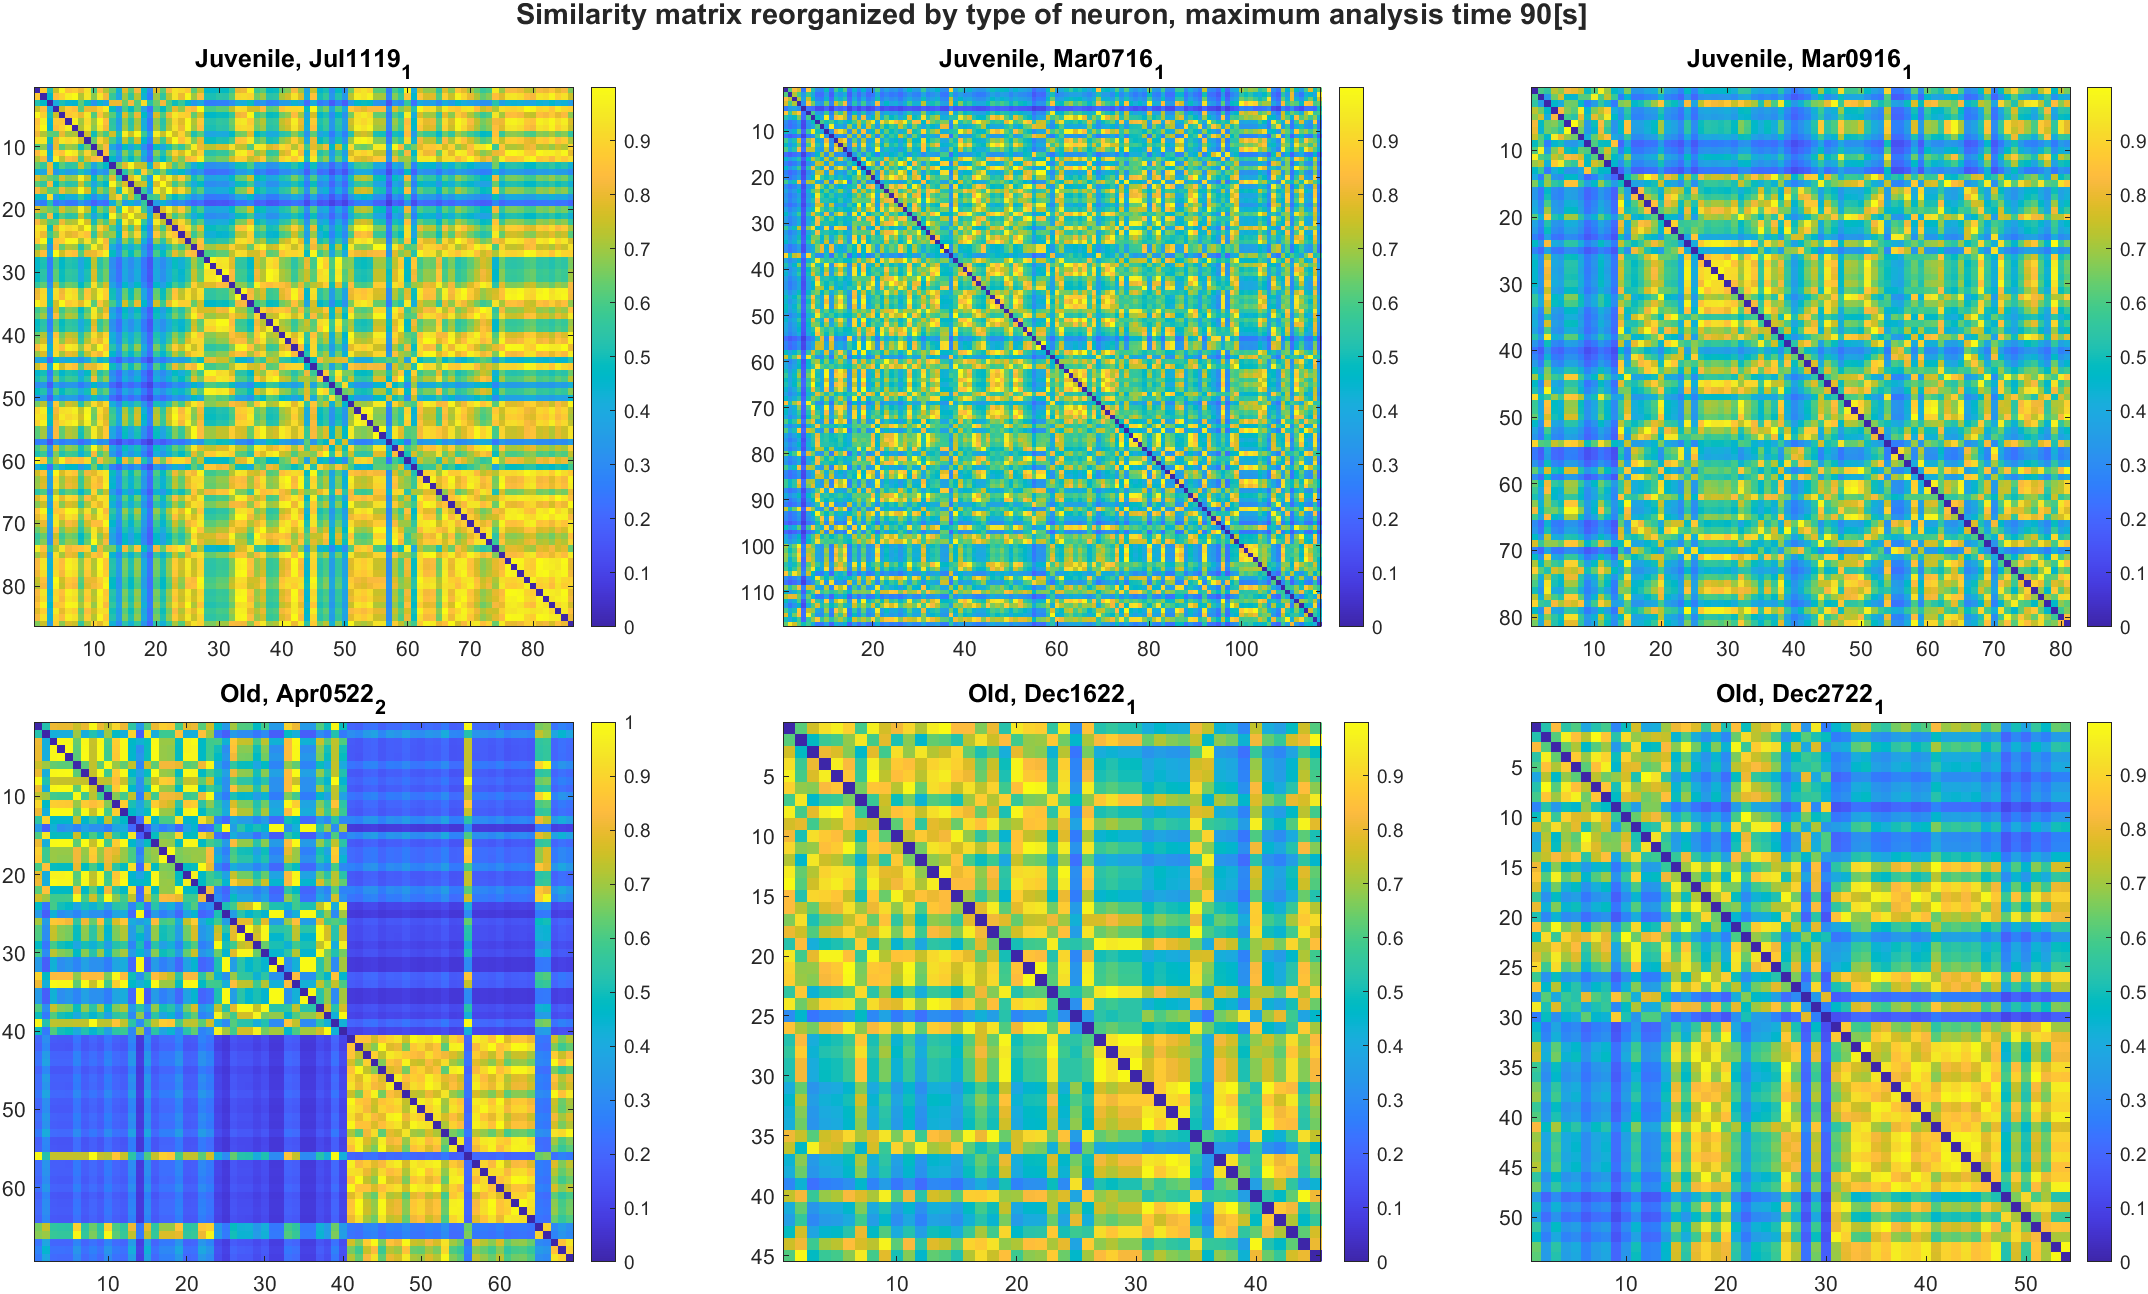
\includegraphics[width=0.8\textwidth]{img/CSM_reorganized.png}}
    
    \caption{Matriz de similaridad del coseno antes y despúes de clasificar las neuronas según patrón de disparo por set de datos.}
    
    \label{csm}
\end{figure}

\begin{figure}
    \centering
    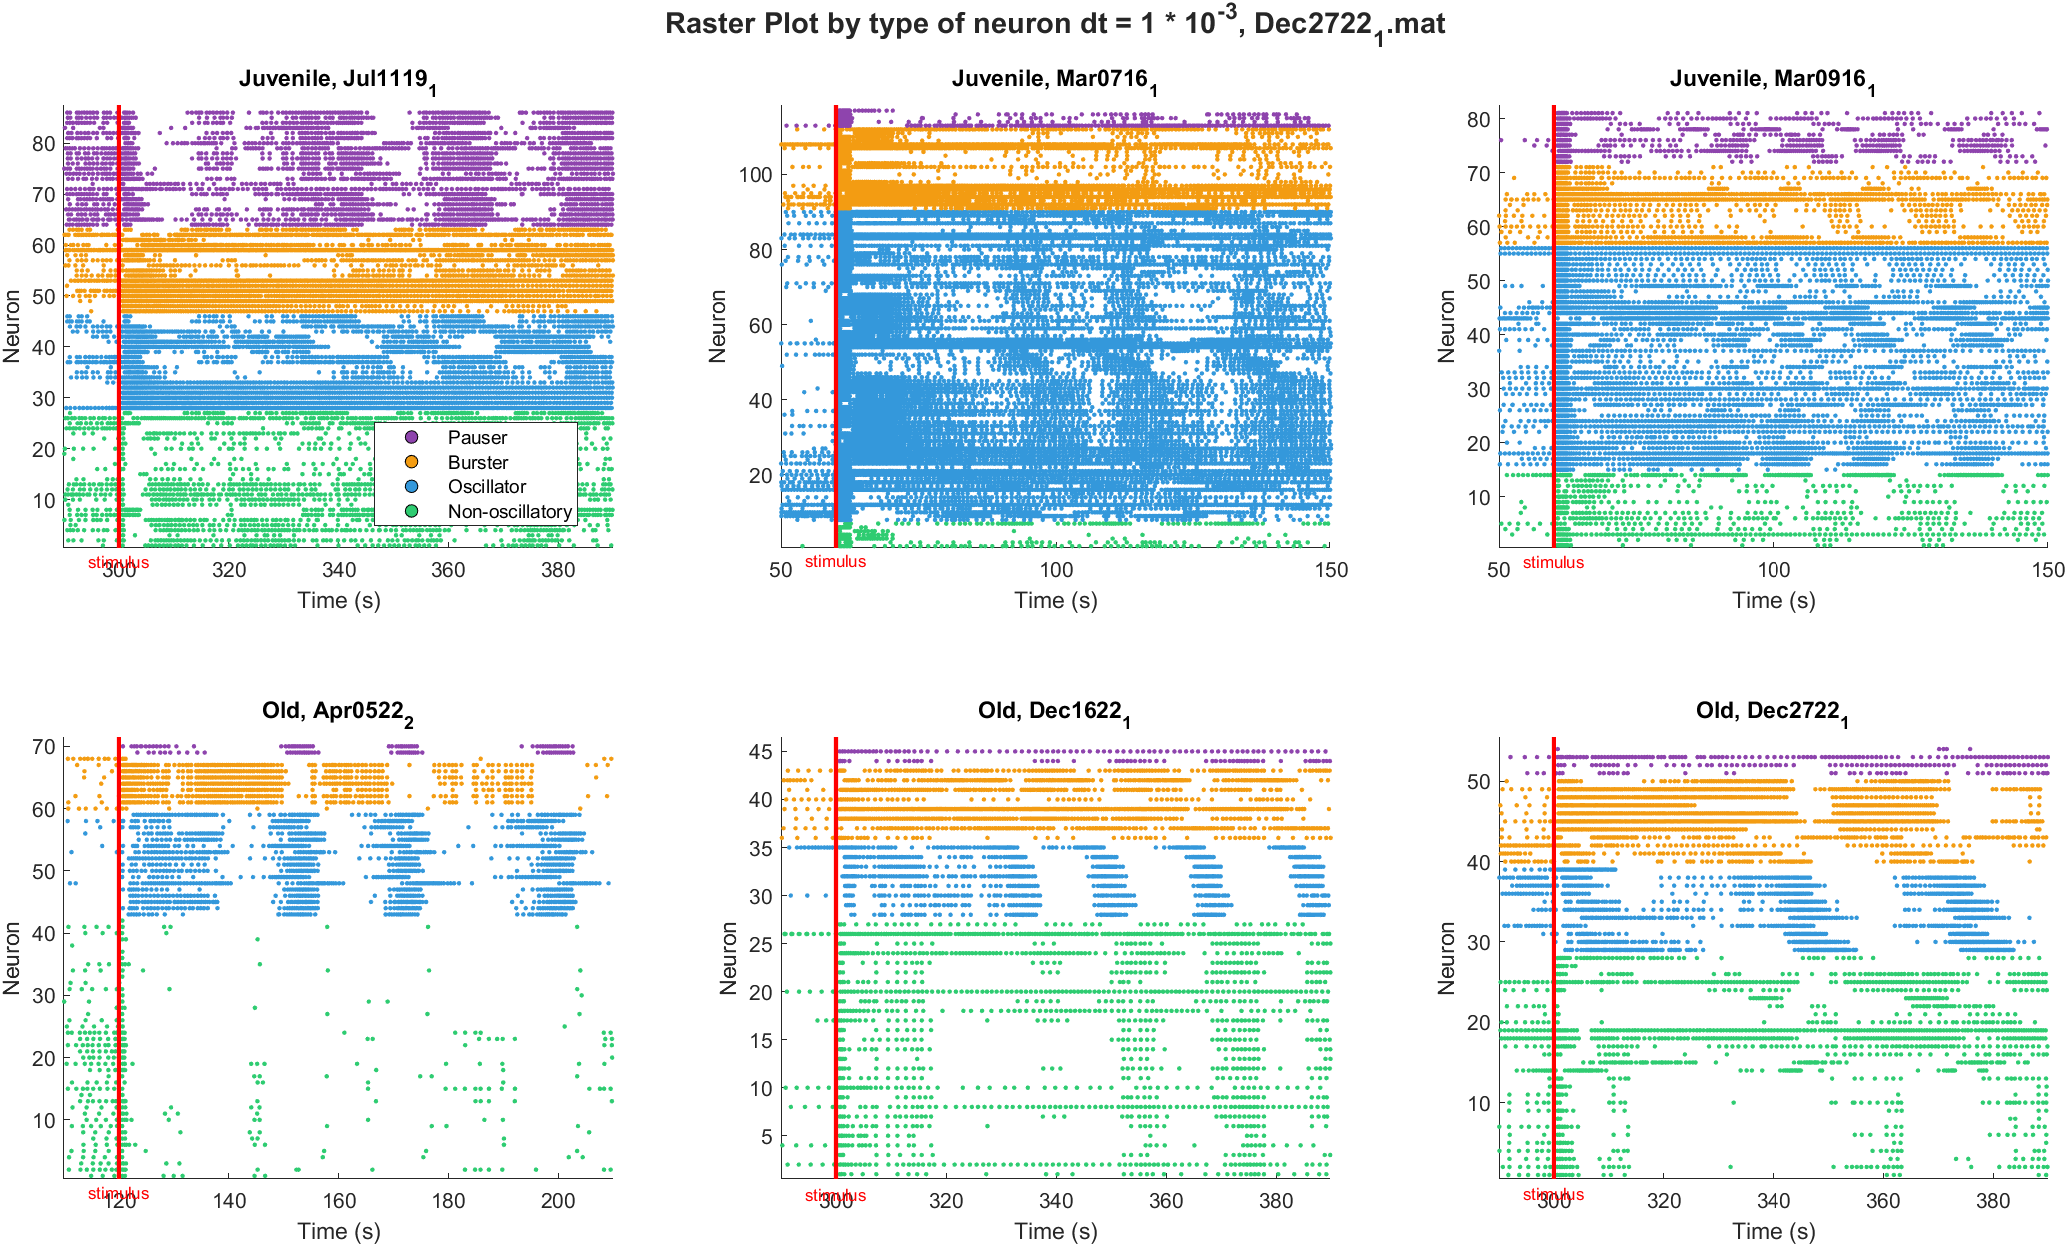
\includegraphics[width=0.7\textwidth]{img/RasterPlot_by_Type.png}
    \caption{Raster Plot con neuronas agrupadas según patrón de oscilación por set de datos.}    
    \label{RP por tipo}
\end{figure}


\begin{figure}
    \centering
    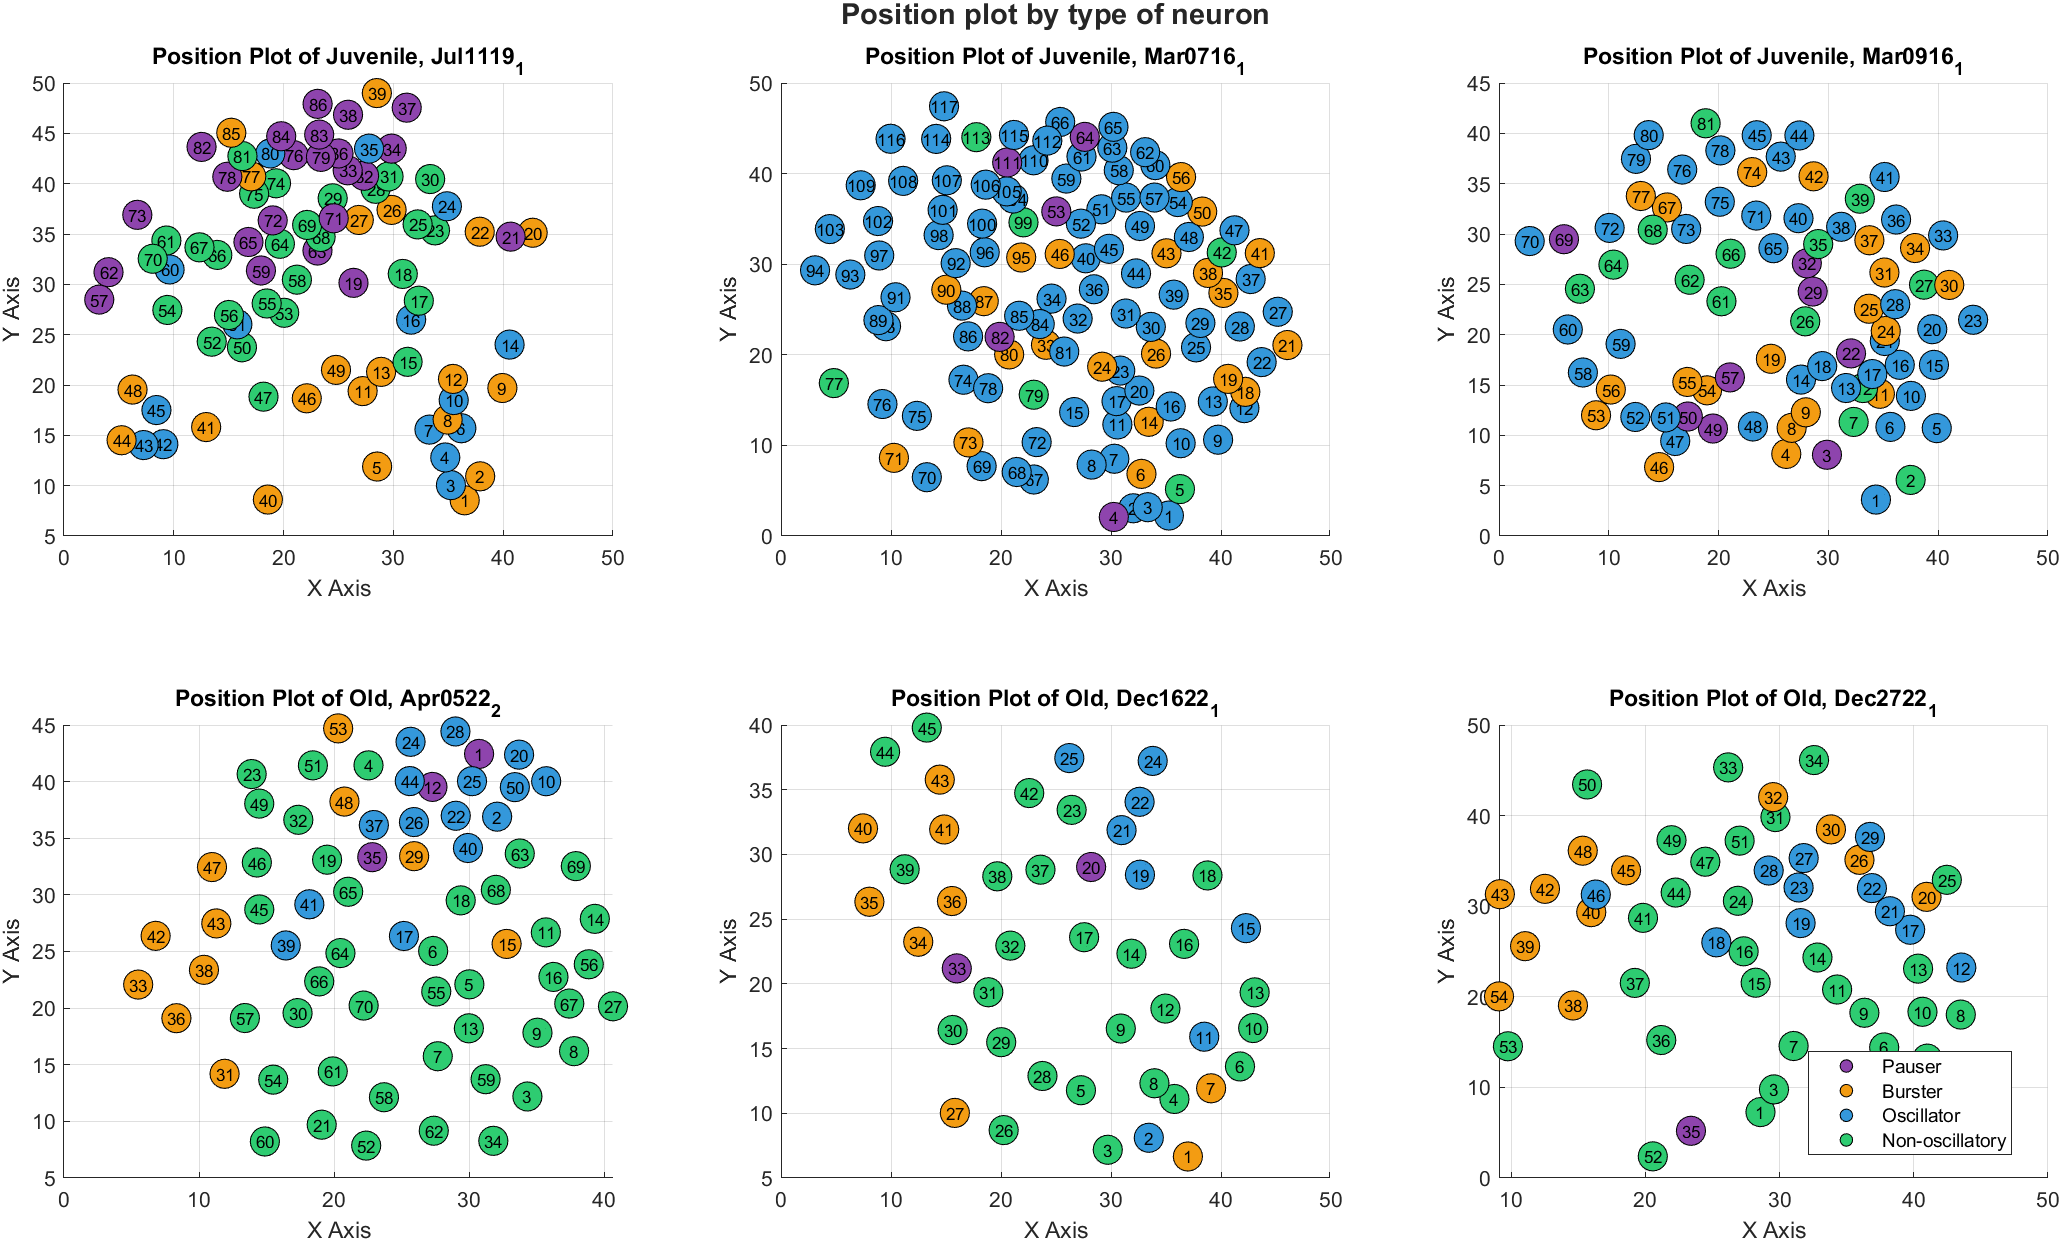
\includegraphics[width=0.7\textwidth]{img/PositionPlot_by_Type.png}
    \caption{Gráfico de posición de neuronas por dataset.}    
    \label{Positionplot}
\end{figure}


Del trabajo realizado se concluye que, al comparar la población joven y envejecida de \textit{Aplysia}, la cantidad total de neuronas disminuye en promedio un 40\%, el promedio de spikes por tiempo, normalizado por el total de neuronas, se reduce en un 50\%, y la cantidad de neuronas oscilatorias disminuye en un 61\%. En este contexto, las neuronas no oscilatorias aumentan, mientras que las demás se mantienen en un rango similar. Finalmente, la posición relativa de los diferentes tipos de neuronas no es concluyente.\\

Todos los códigos utilizados se encuentran en el Github <\url{https://github.com/JavieraRojasM/Practica.git}> .

\clearpage

% \begin{references}


%     \bibitem{bib perdida sinaptica}
%     Etan J. Markus, Ted L. Petit. Neocortical synaptogenesis, aging, and behavior: Lifespan development in the motor-sensory system of the rat. 1987. [en línea] <\url{https://www.sciencedirect.com/science/article/pii/0014488687900458}>

%    \bibitem{bib burst}
%    Ishida, Y., Kozaki, T., Isomura, Y., Ito, S., Isobe, Ki. Age-Dependent Changes in Dopaminergic Neuron Firing Patterns in Substantia Nigra Pars Compacta. 2009. [en línea] <\url{https://link.springer.com/chapter/10.1007/978-3-211-92660-4_10}>

%     \bibitem{bib Ca}
%     Thomas A. Pitler, Philip W. Landfield. Aging-related prolongation of calcium spike duration in rat hippocampal slice neurons. 1990. [en línea]<\url{https://www.sciencedirect.com/science/article/pii/000689939091109T?ref=pdf_download&fr=RR-2&rr=8fc2a2a4af8988a6}>
    
%    \bibitem{bib Potasio}
%     B. Potier, O. Rascol, F. Jazat, Y. Lamour, P. Dutar. Alterations in the properties of hippocampal pyramidal neurons in the aged rat. 1992. [en línea] <\url{https://www.sciencedirect.com/science/article/pii/0306452292902676}>
    
%     \bibitem{bib sensoriales}
%     Kempsell Andrew T. , Fieber Lynne A. Behavioral aging is associated with reduced sensory neuron excitability in Aplysia californica. 2014. [en línea] <\url{https://www.frontiersin.org/journals/aging-neuroscience/articles/10.3389/fnagi.2014.00084/full}>

%    \bibitem{bib cantidad}
%     Bertram Peretz, Malathi Srivatsan. Differences in aging in two neural pathways: Proposed explanations from the nervous system of aplysia. 1992. [en línea] <\url{https://www.sciencedirect.com/science/article/pii/053155659290031T}>
    
%    \bibitem{AMB}
%     Angela M. Bruno, William N. Frost, Mark D. Humphries. Modular Deconstruction Reveals the Dynamical and Physical Building Blocks of a Locomotion Motor Program. 2015. [en línea] <\url{https://www.sciencedirect.com/science/article/pii/S0896627315002019?via%3Dihub}>

% \end{references}
 % Ejemplo, se puede borrar

\section{Descripción del ámbito productivo en el que se realiza la PPII }

La Práctica Profesional II fue realizada en el Departamento de Neurociencia de la Facultad de Medicina de la Universidad de Chile. Específicamente, se llevó a cabo en la línea de investigación en neuromodulación y control motor, dirigida por el Dr. Rómulo Fuentes.\\

El departamento se dedica principalmente a la investigación científica, contando con diversas líneas en las que trabajan investigadores enfocados en distintas temáticas dentro del ámbito de la neurociencia.\\

El trabaj de práctica se desarrolló bajo la supervisión de la Dra. Andrea Colins y tuvo como objetivo el análisis de datos de actividad neuronal del ganglio pedal de ejemplares jóvenes y de mayor edad de Aplysia. Para ello, se aplican métodos estadísticos con el fin de comparar la actividad neuronal entre ambos grupos etarios.\\

Entre los insumos utilizados se incluye un computador con el rendimiento necesario para procesar grandes volúmenes de datos, una licencia estudiantil de MATLAB proporcionada por la Universidad de Chile y los registros neuronales, los cuales fueron facilitados por la Dra. Andrea Colins.\\

Los datos entregados corresponden a seis grabaciones en total: tres de Aplysia jóvenes y tres de Aplysia de mayor edad. Cada grabación contenía un archivo con la posición espacial de cada neurona, y otro con los tiempos en que cada una genera un spike.\\

\section{Descripción de la(s) tarea(s) ejecutadas durante la PPII}


Se inicia con una búsqueda bibliográfica sobre estudios similares tanto en mamíferos como en \textit{Aplysia}, de la cual se identifican experimentos similares en ratas, donde las principales conclusiones indican que, con la edad, ocurre una pérdida de densidad sináptica \cite{bib perdida sinaptica}, un aumento de la cantidad de neuronas con patrones de disparo tipo burst \cite{bib burst}, un aumento de la conductancia de calcio en canales dependientes de voltaje \cite{bib Ca}, facilitando la generación de spikes y, finalmente, una reducción en la conductancia de potasio en canales dependientes de voltaje \cite{bib Potasio}, lo que prolonga la duración del spike.\\

Por otra parte, en \textit{Aplysia} se ha observado una relación entre el envejecimiento conductual y la disminución de la excitabilidad en las neuronas sensoriales \cite{bib sensoriales}, además de una reducción en la cantidad de spikes y un aumento en su duración sin cambio en el intervalo existente entre spikes \cite{bib cantidad}.\\

Luego de la búsqueda bibliográfica, se realiza un análisis estadístico neuronal estándar, donde se reduce el tiempo de grabación a un máximo de 90 segundos tras la aplicación del estímulo y se grafica, por grupo etario, el total de neuronas, los Raster plot correspondientes y el promedio global de spikes por tiempo y por neurona.\\

En neuronciencia, los Raster plot son gráficos ampliamente utiliados para visualizar la actividad neuronal en el tiempo. Cada línea horizontal representa una neurona y las marcas indican los momentos en que ocurren los spikes. Este tipo de gráfico permite identificar patrones de activación, sincronización entre neuronas y respuestas a estímulos de forma clara y concisa.\\


Luego de este primer análisis estadístico, se propone como hipótesis que la diferencia entre la actividad neuronal de los dos grupos etarios radica en la cantidad de neuronas que tienen un patrón de disparo similar, por lo que se propone como metodología realizar un análisis similar al propuesto en el paper \textit{``Modular Deconstruction Reveals the Dynamical and Physical Building Blocks of a Locomotion Motor Program''} \cite{AMB} publicado en 2015, para clasificar las neuronas según su patrón de disparo. La clasificación se basa en la correlación cruzada de los spikes train discretizados junto con una prueba de permutación. \\

Con las neuronas clasificadas según su tipo de disparo, se analiza la cantidad de neuronas de cada tipo utilizando un gráfico circular. Además, se grafica la matriz de similitud del coseno antes y después de la clasificación para comprobar el éxito del agrupamiento. Posteriormente, se generan nuevamente los raster plots, esta vez con las neuronas agrupadas por tipo, y finalmente, se realiza un gráfico de posición donde cada tipo de neurona se representa con un color diferente.\\
\newpage
\section{Resultados y conclusiones principales}


De la metodología anterior, se obtienen los siguientes resultados.\\

\begin{figure}
    \centering
    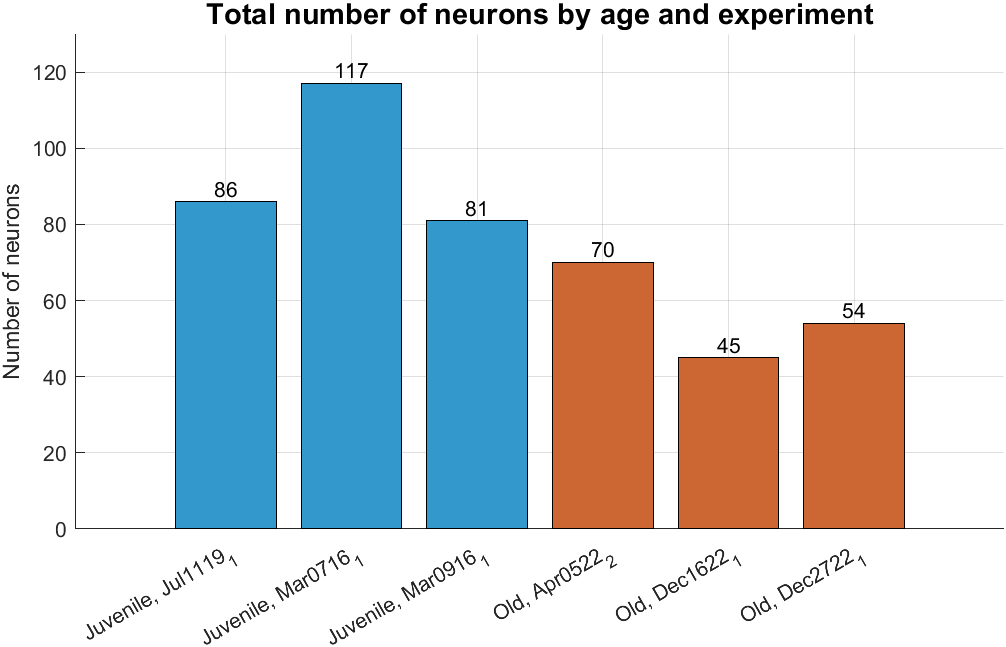
\includegraphics[width=0.6\textwidth]{img/Total_Neurons.png}
    \caption{Total de neuronas por set de datos.}
    \label{total_neurons}
\end{figure}

\begin{figure}
    \centering
    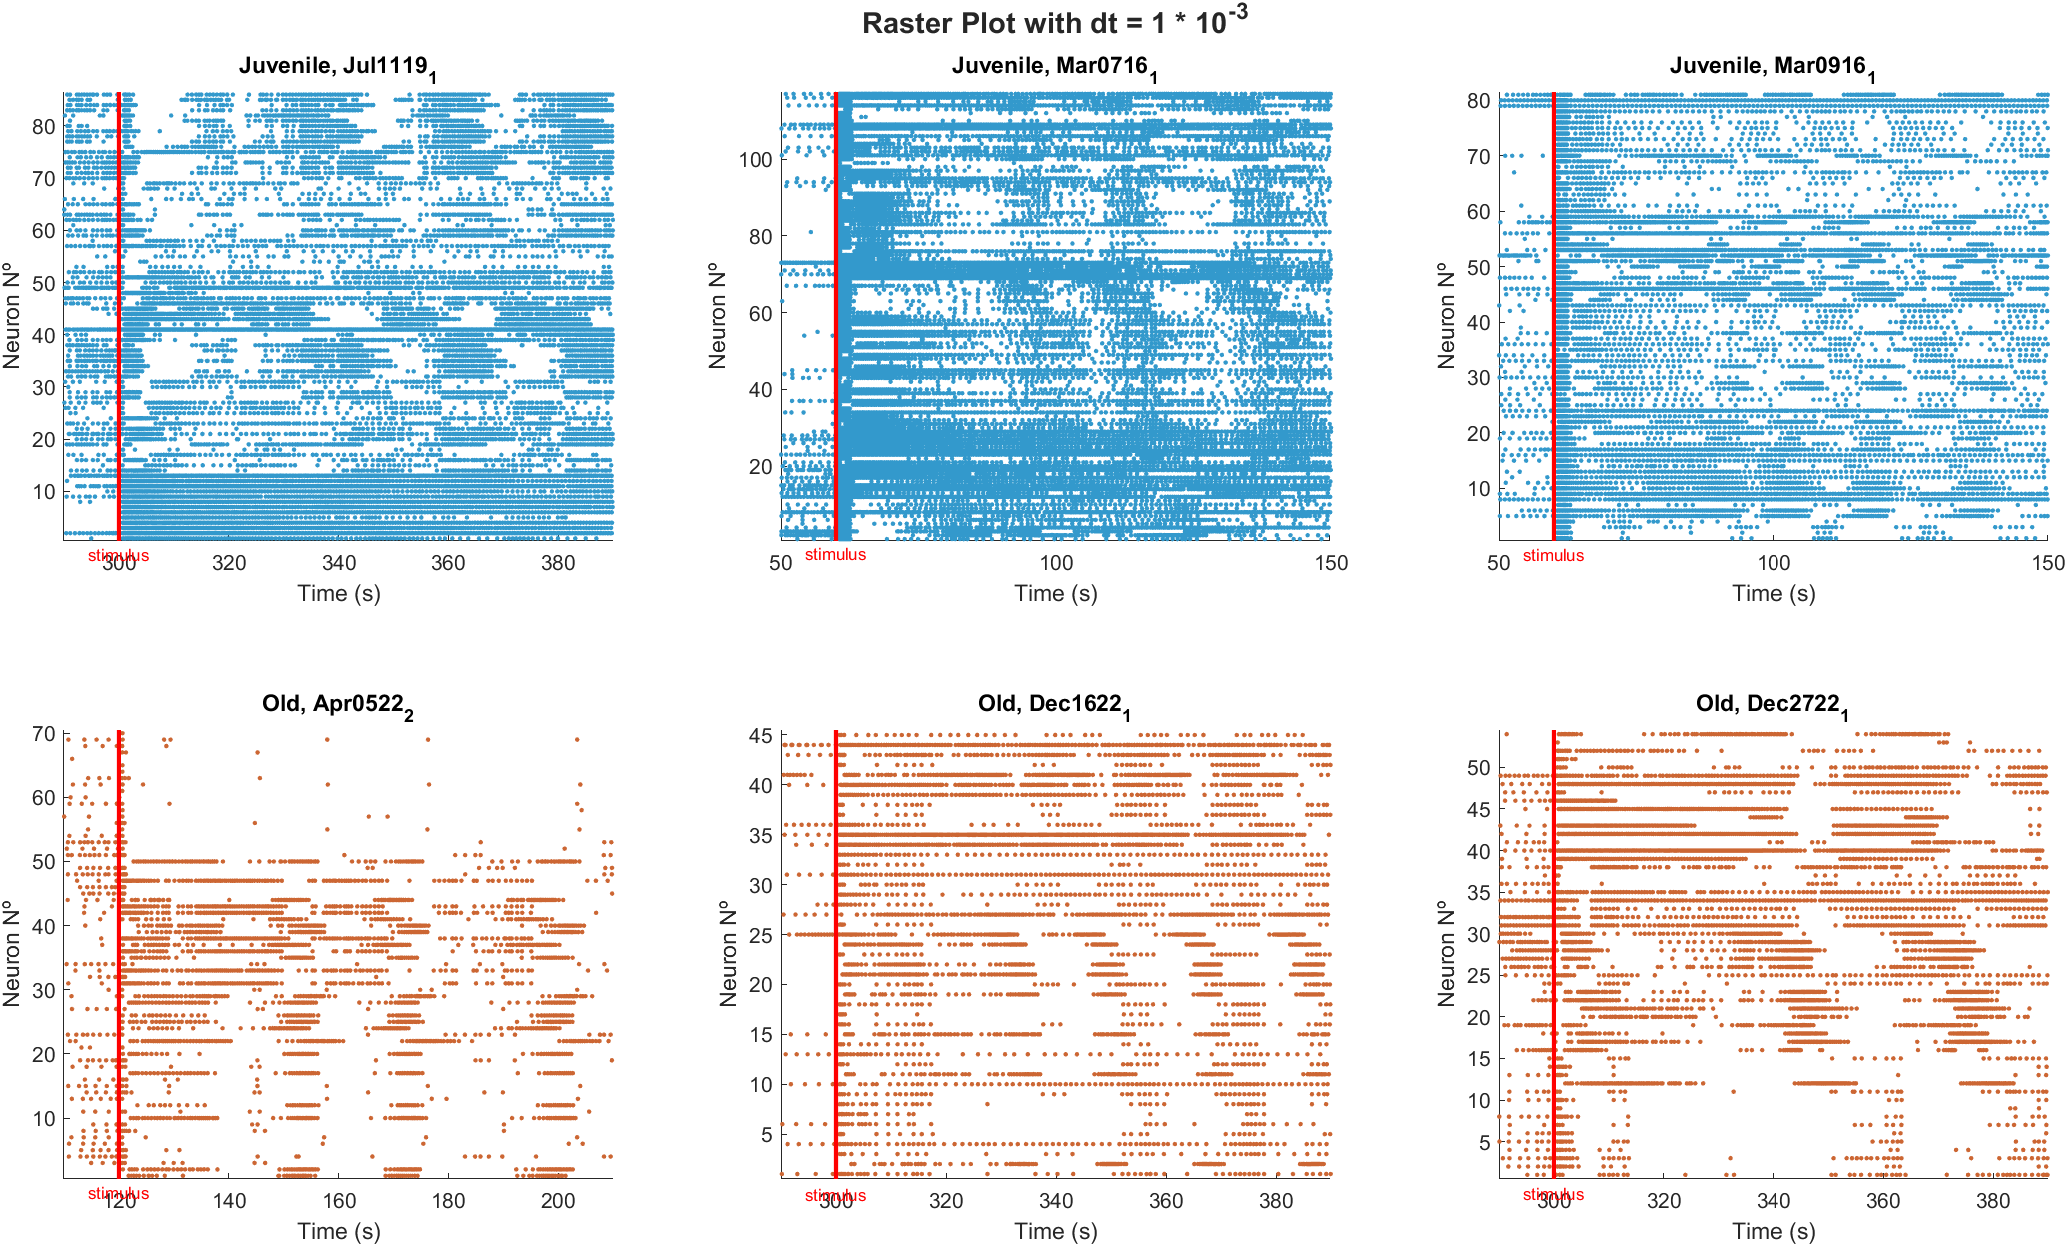
\includegraphics[width=0.9\textwidth]{img/RasterPlot.png}
    \caption{Raster Plot por set de datos.}    
    \label{rasterplot}
\end{figure}

\begin{figure}
    \centering
    \subfloat{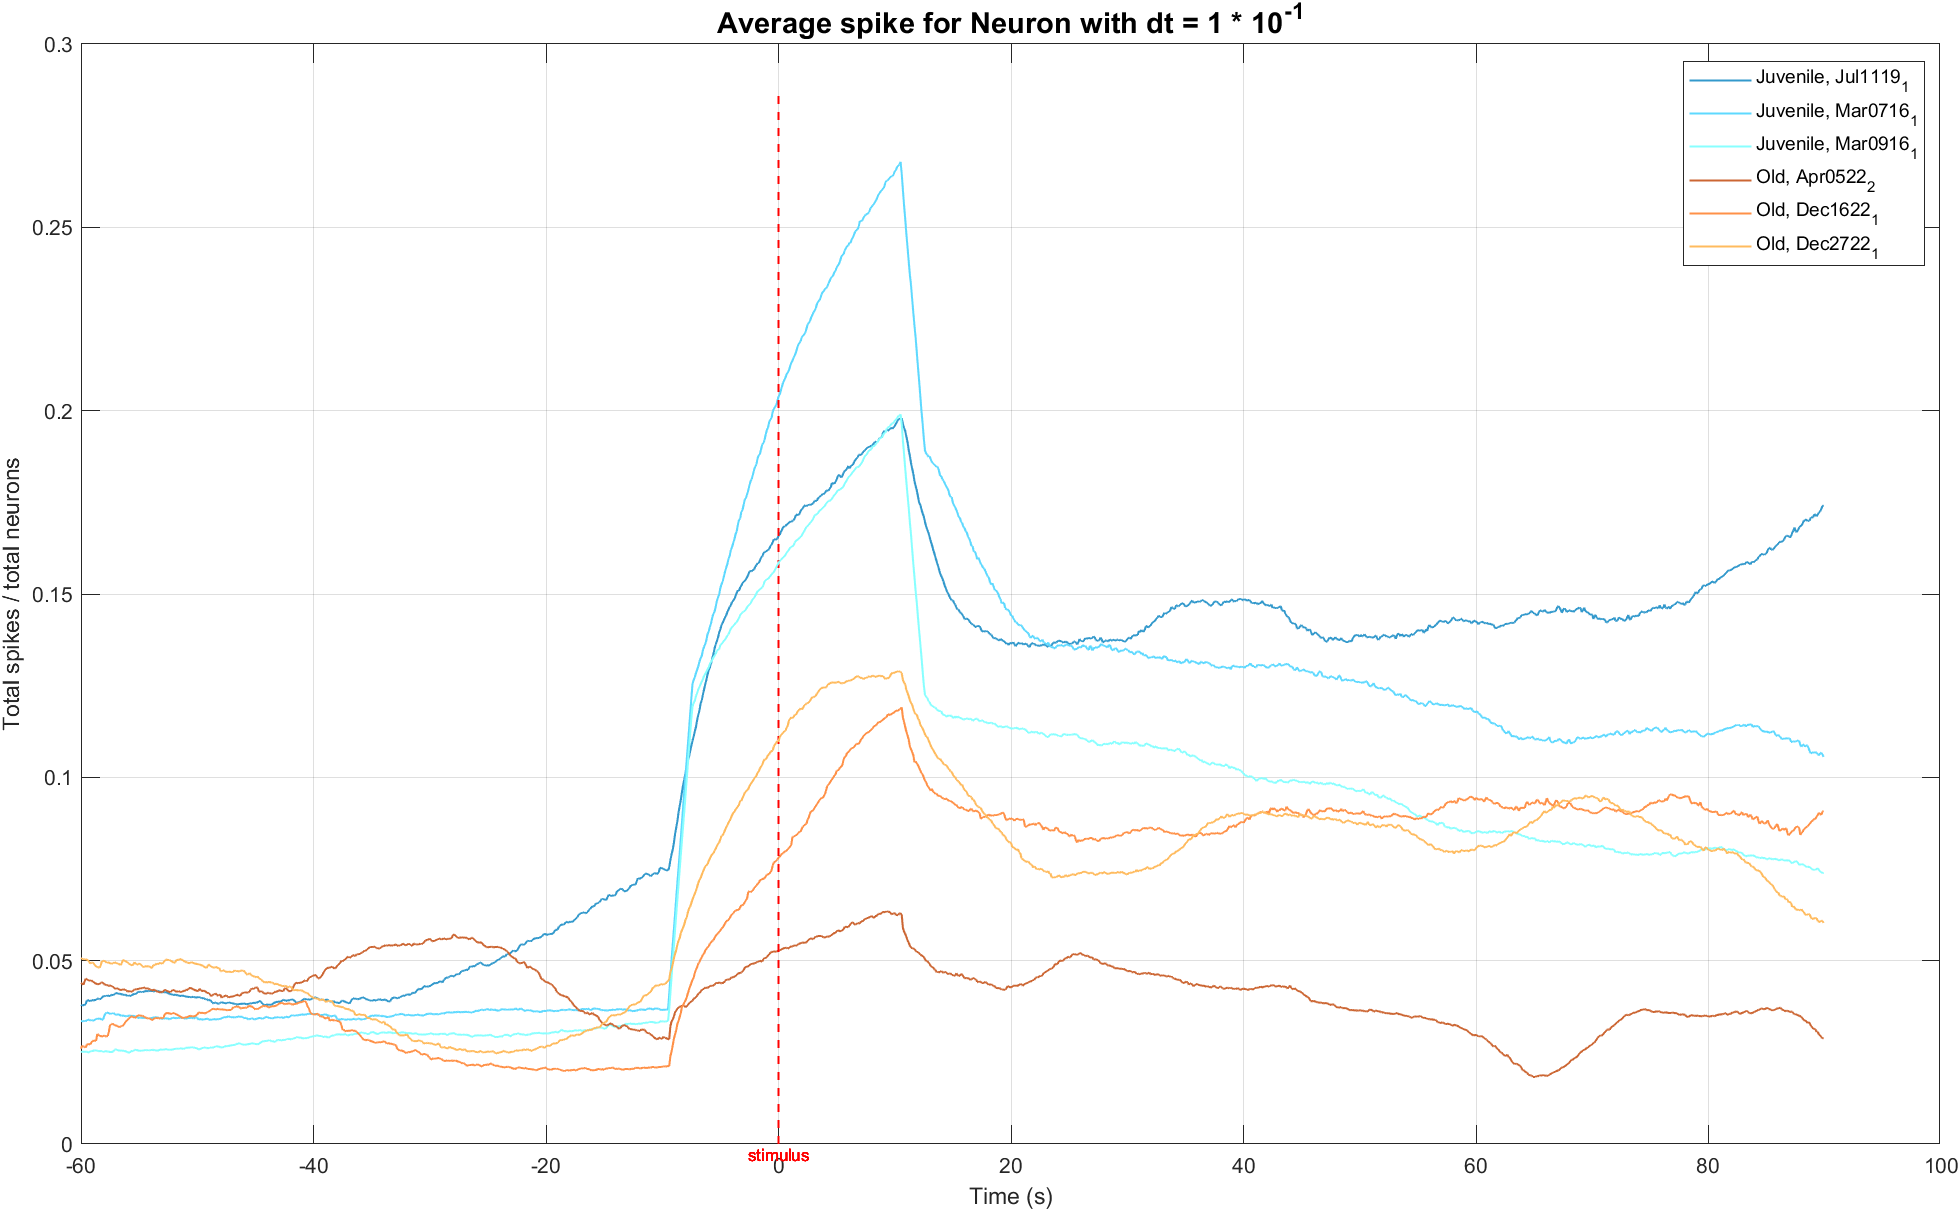
\includegraphics[width=0.8\textwidth]{img/Average_spike_for_Neuron.png}}
    
    \hfill
    
    \subfloat{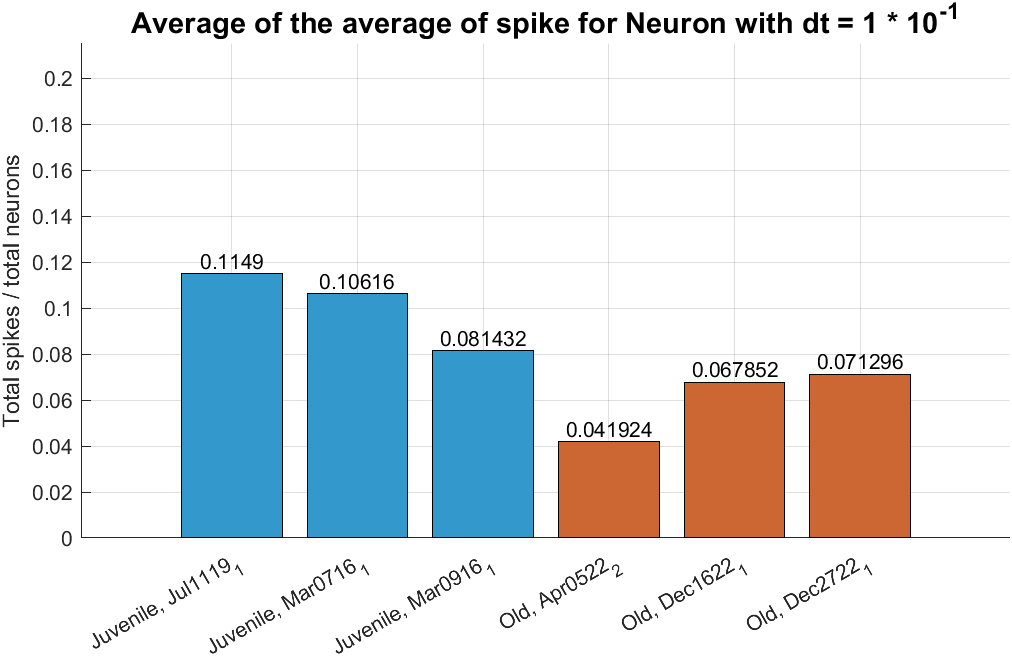
\includegraphics[width=0.7\textwidth]{img/Average_of_the_average_spike_for_Neuron.png}}
    
    \caption{Promedio de spikes totales normalizado por cantidad total de neuronas por set de datos.}
    
    \label{promdelprom}
\end{figure}

\begin{figure}
    \centering
    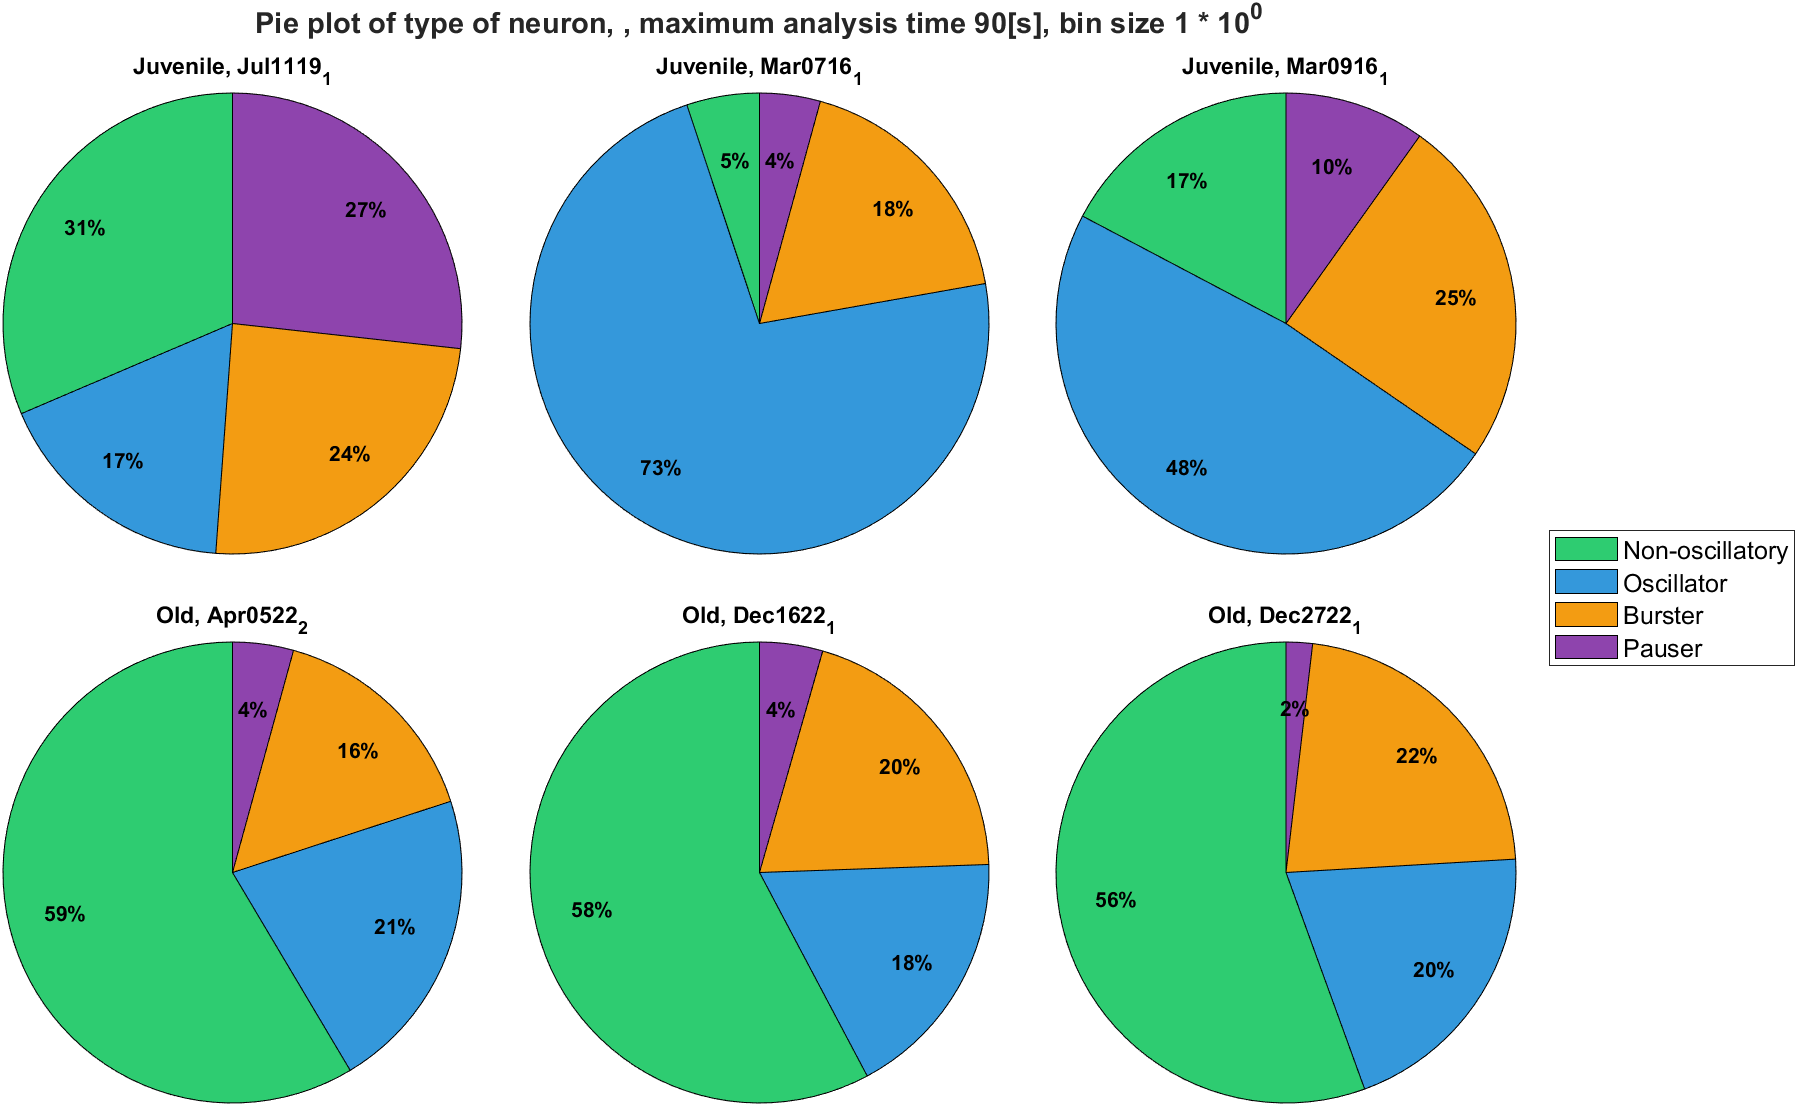
\includegraphics[width=0.7\textwidth]{img/Pie_plot_of_type_of_Neuron.png}
    \caption{Gráfico circular de total de neuronas de cada tipo por set de datos.}    
    \label{pieplot}
\end{figure}

\begin{figure}
    \centering
    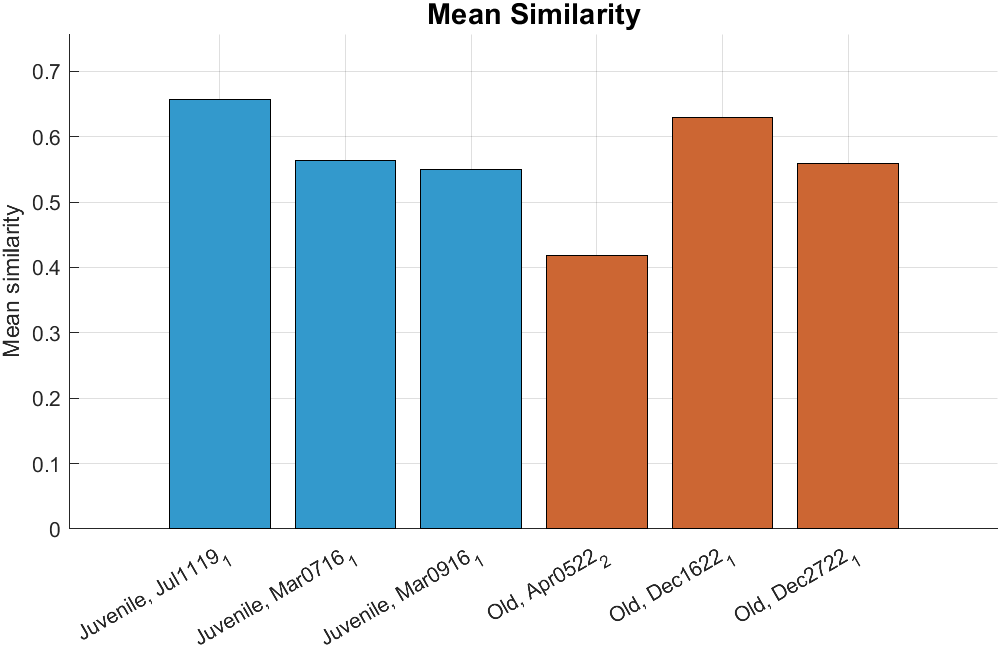
\includegraphics[width=0.7\textwidth]{img/Mean_similarity.png}
    \caption{Promedio de similaridad en matrix de similaridad del coseno por set de datos.}    
    \label{pieplot}
\end{figure}


\begin{figure}
    \centering
    \subfloat{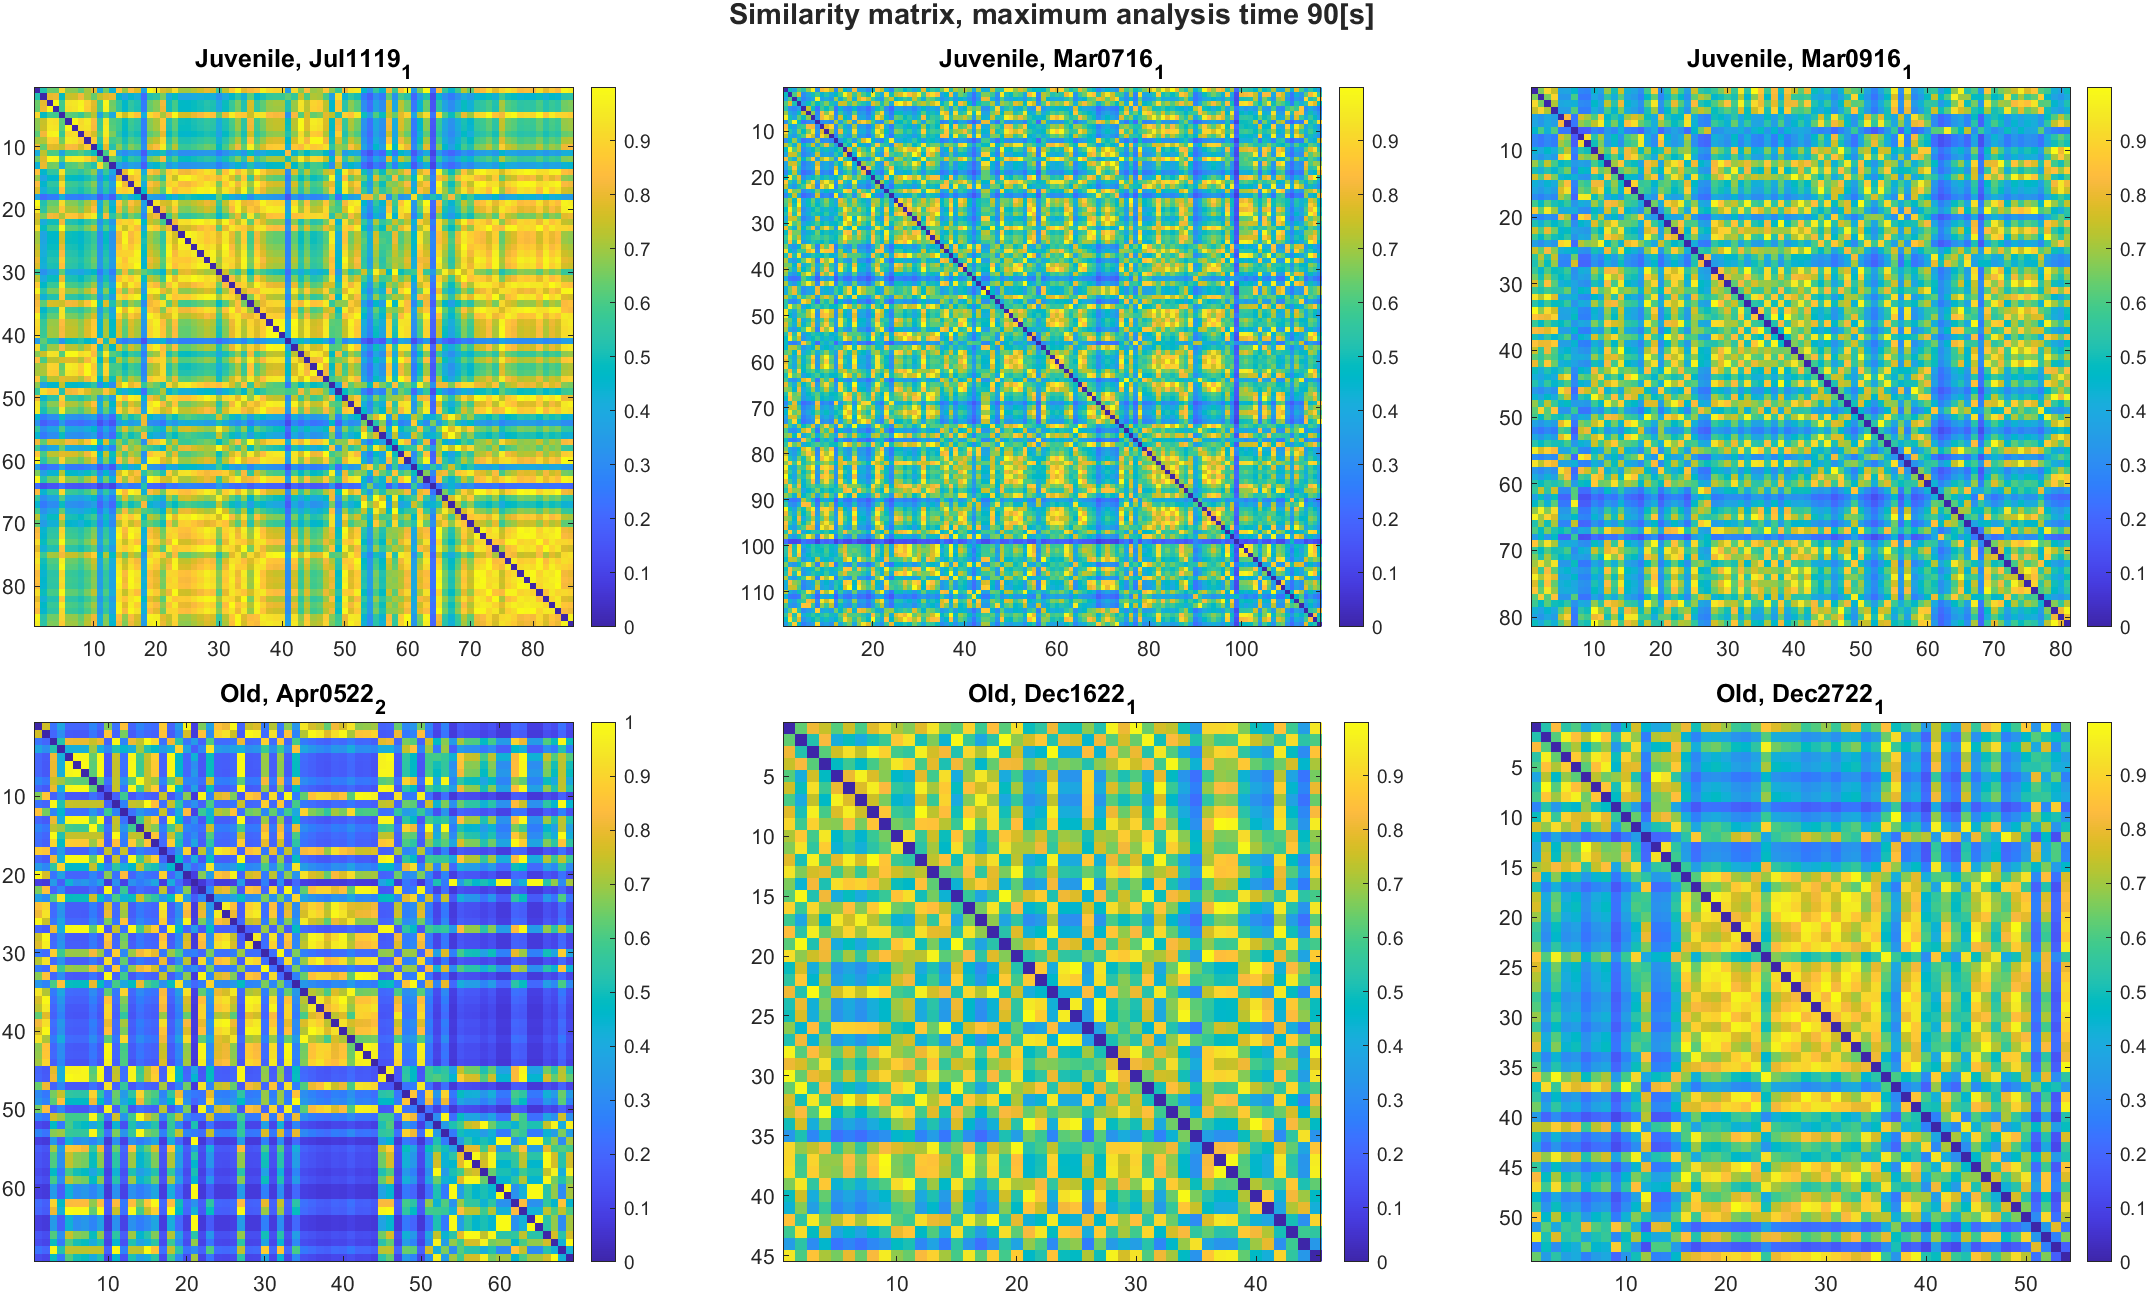
\includegraphics[width=0.9\textwidth]{img/CSM_base.png}}
    
    \hfill
    
    \subfloat{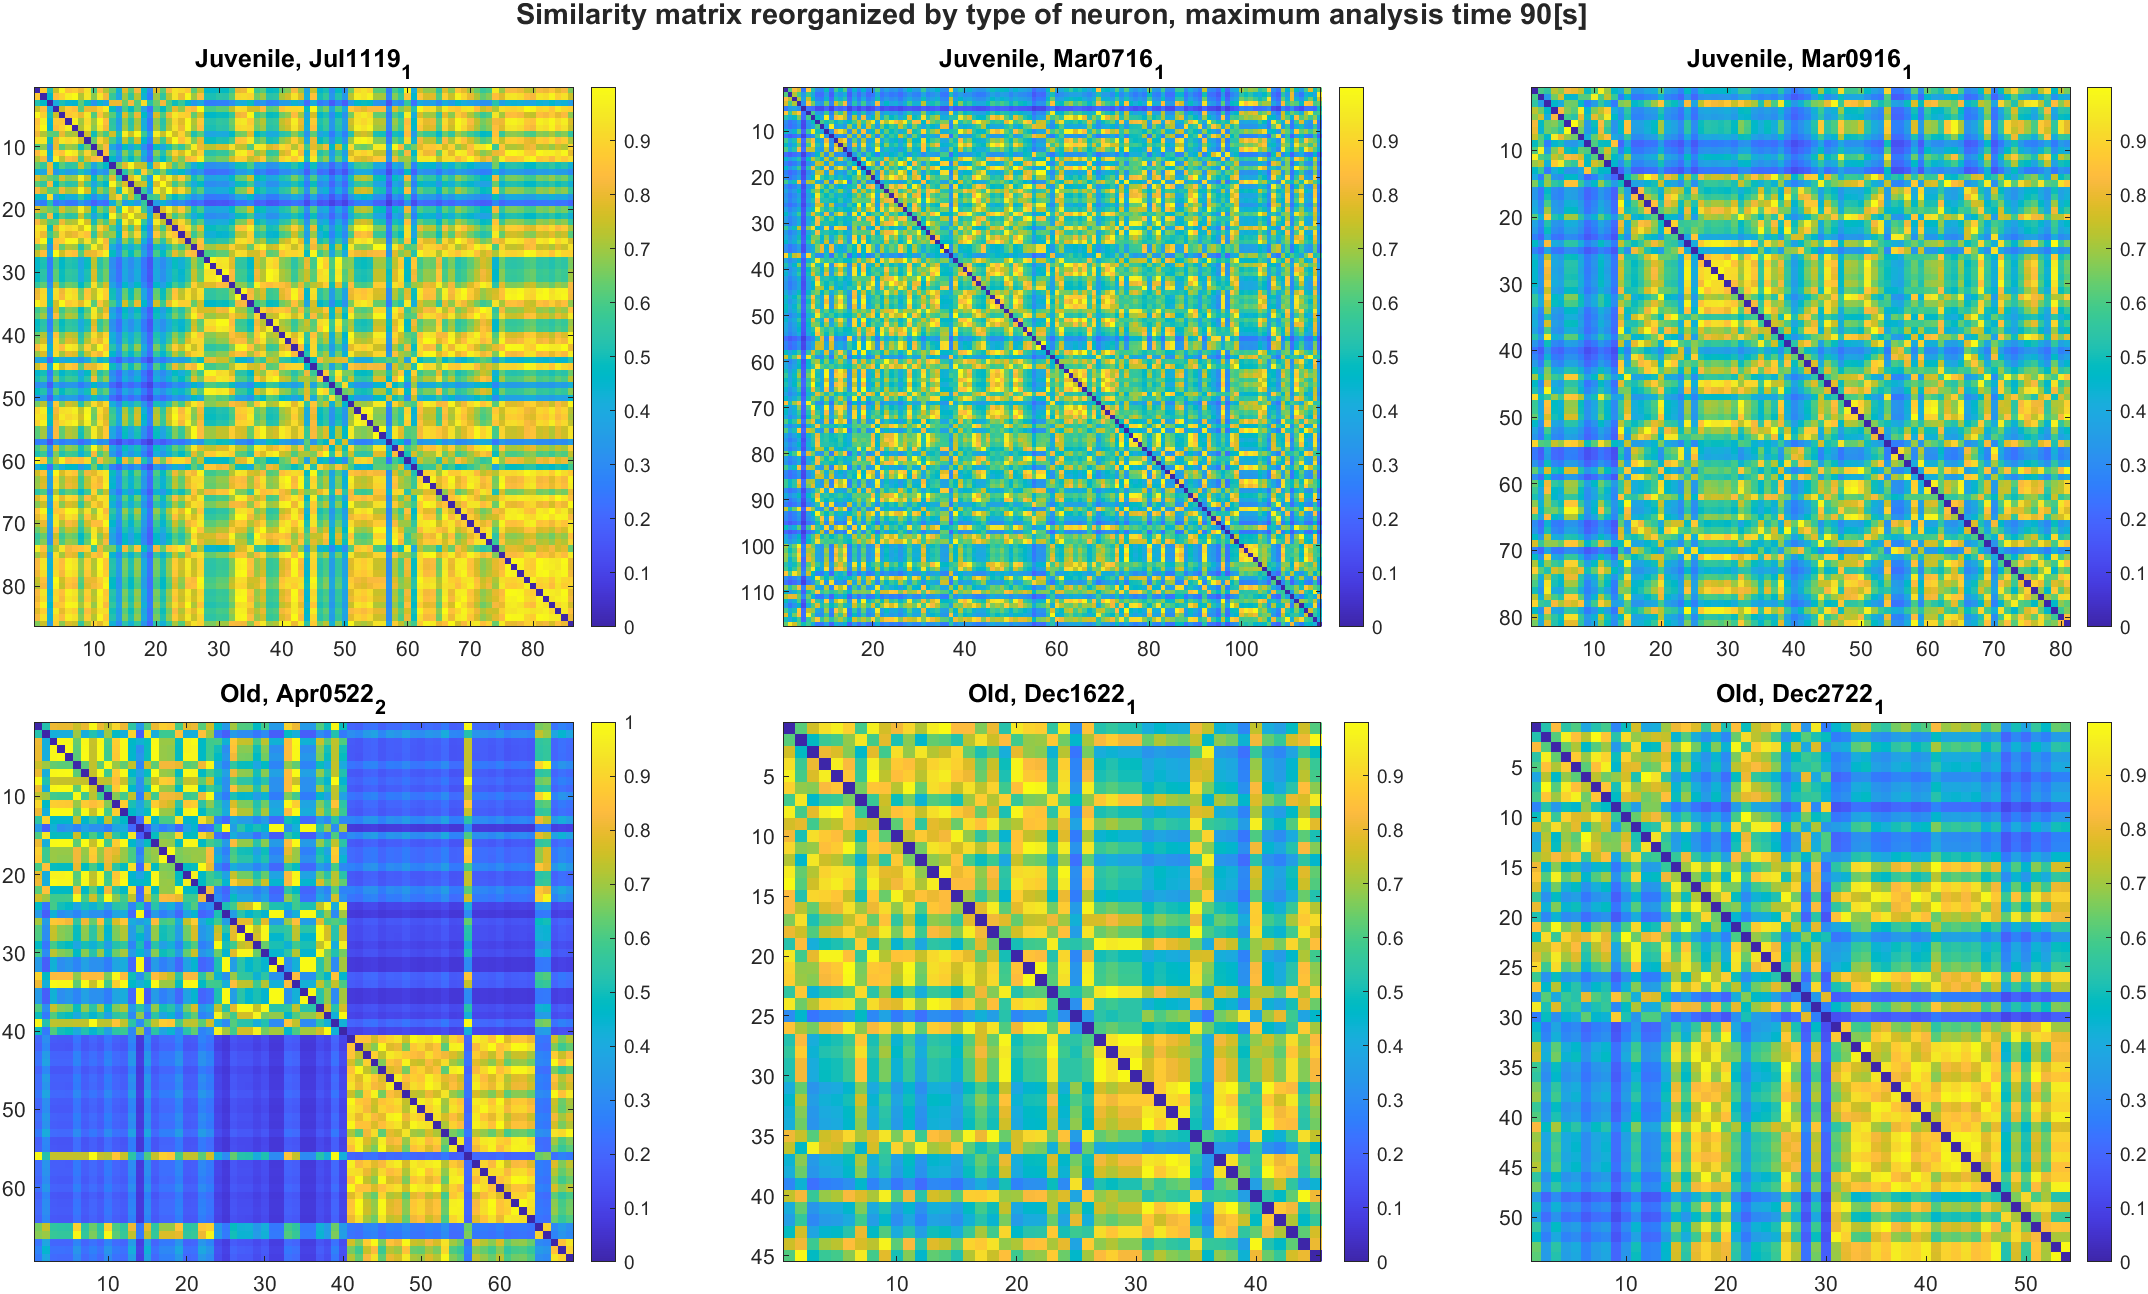
\includegraphics[width=0.9\textwidth]{img/CSM_reorganized.png}}
    
    \caption{Matriz de similaridad del coseno antes y despúes de clasificar las neuronas según patrón de disparo por set de datos.}
    
    \label{csm}
\end{figure}

\begin{figure}
    \centering
    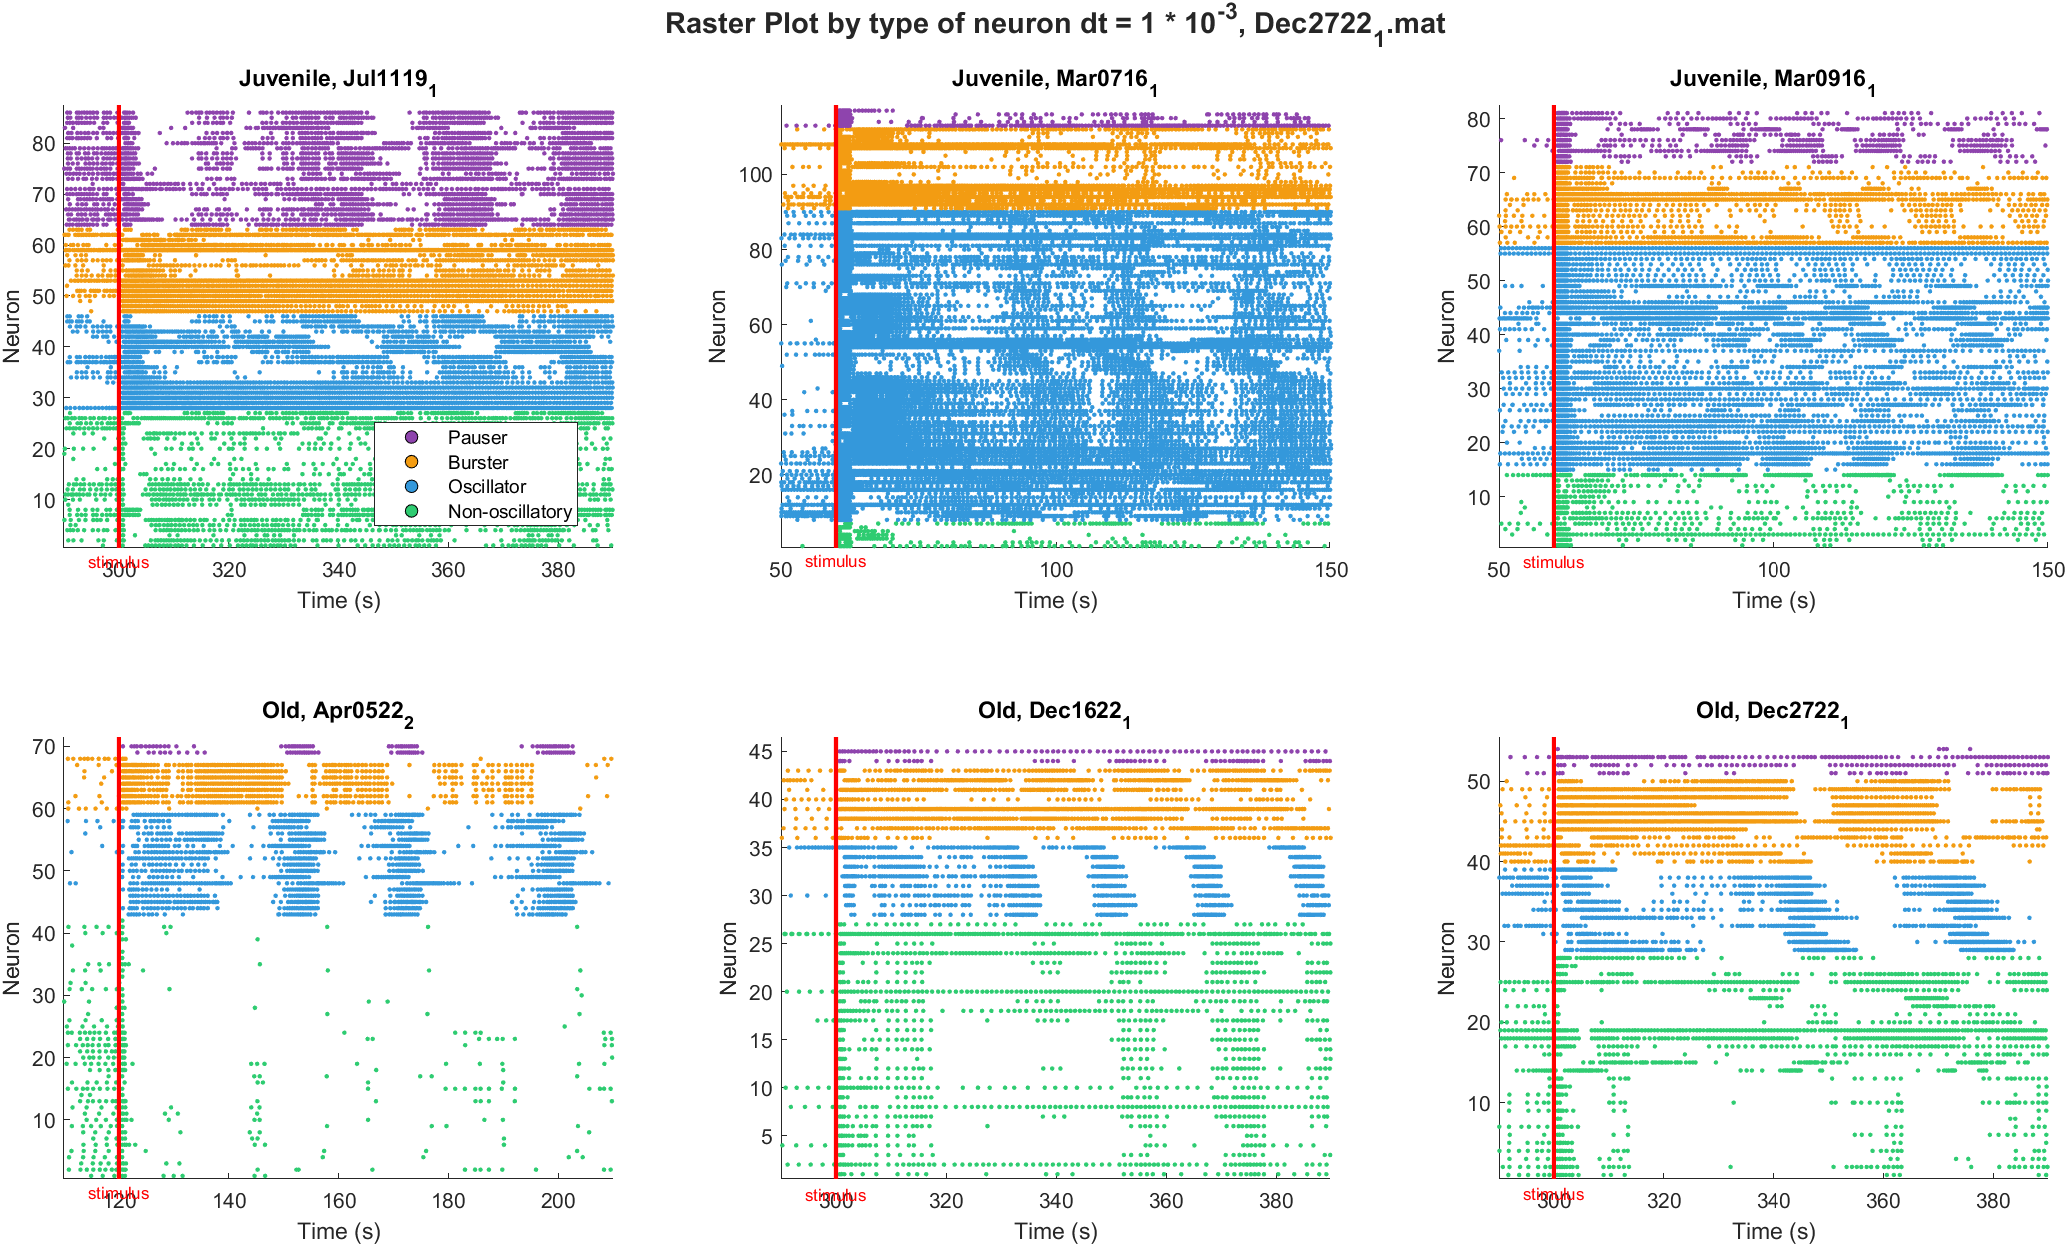
\includegraphics[width=0.9\textwidth]{img/RasterPlot_by_Type.png}
    \caption{Raster Plot con neuronas agrupadas según patrón de oscilación por set de datos.}    
    \label{RP por tipo}
\end{figure}


\begin{figure}
    \centering
    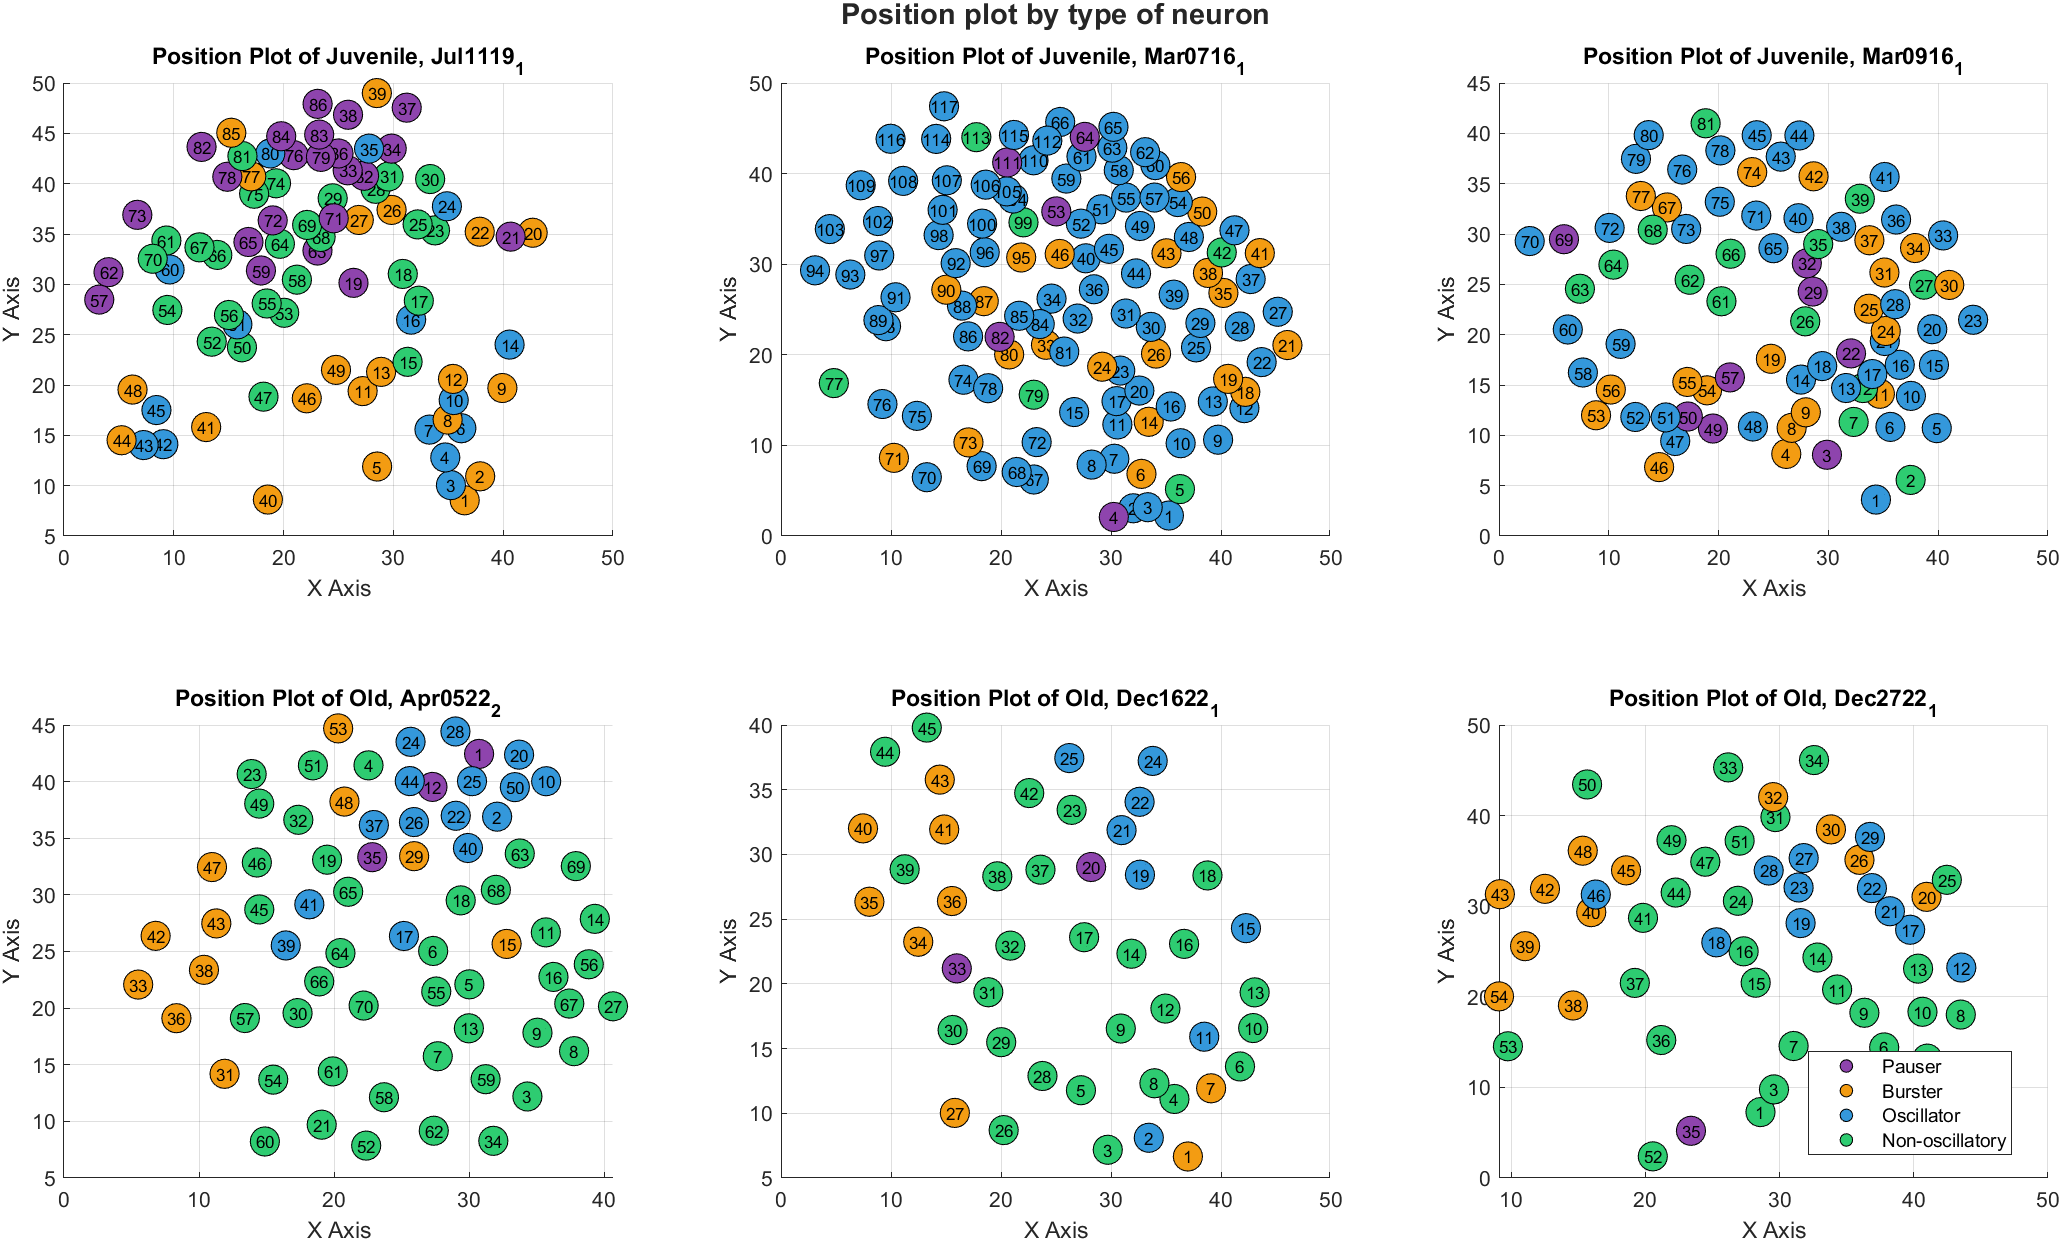
\includegraphics[width=0.9\textwidth]{img/PositionPlot_by_Type.png}
    \caption{Gráfico de posición de neuronas por dataset.}    
    \label{Positionplot}
\end{figure}

\newpage
Del trabajo realizado se concluye que, al comparar la población joven y envejecida de \textit{Aplysia}, la cantidad total de neuronas disminuye en promedio un 40\%, el promedio de spikes por tiempo, normalizado por el total de neuronas, se reduce en un 50\%, y la cantidad de neuronas oscilatorias disminuye en un 61\%. En este contexto, las neuronas no oscilatorias aumentan, mientras que las demás se mantienen en un rango similar. Finalmente, la posición relativa de los diferentes tipos de neuronas no es concluyente.\\

Se obtiene además como resultado, una carpeta de Github <\url{https://github.com/JavieraRojasM/Practica.git}> con todos los códigos de Matlab necesarios para realizar un análisis estadístico estándar de actividad neuronal y un archivo README.txt el cual contiene las instrucciones de uso de los códigos.
\section{Limitaciones, aspectos positivos y recomendaciones al proceso productivo}

Las principales limitaciones identificadas durante la práctica, se encuentra la disponibilidad de recursos y de datos. En cuanto a los recursos, uno de los principales obstáculos surgie al intentar replicar el análisis estadístico descrito en el paper \textit{Modular Deconstruction Reveals the Dynamical and Physical Building Blocks of a Locomotion Motor Program} (2015) \cite{AMB}. Este estudio utiliza \textit{toolboxes} que no están disponibles en la licencia estudiantil de MATLAB proporcionada por la universidad, por lo que una gran cantidad de tiempo fue dedicada a programar desde cero varias de las funciones utilizadas.\\

Respecto a la disponibilidad de datos, los resultados obtenidos no son representativos debido al tamaño limitado de la muestra. Además, no se dispone de información detallada sobre la metodología utilizada para la recolección de los datos originales, lo que dificulta su validación y análisis. En particular, los datos de posición espacial de las neuronas dependen de cómo se dispone el ganglio durante la medición, y si bien las neuronas de \textit{Aplysia} son de un tamaño mayor al estándar, siguen siendo lo suficientemente pequeñas para que un poco de variabilidad espacial pueda resultar en que se encuentre en la posición de otra neurona de otra grabación, lo que limita la confiabilidad del análisis realizado.\\

Estas limitaciones impidieron cumplir completamente con la actividad planteada en el plan de práctica: \textit{``Se plantearán diagramas del fenómeno a modelar, utilizando herramientas para el modelamiento tales como MATLAB, y se definirán las ecuaciones para la construcción y formulación del modelo matemático, con base en la fenomenología del proceso a modelar''}, ya que el tiempo disponible para la realización de la práctica . No obstante, se considera que sí se logró avanzar en el desarrollo de la competencia específica CE6: \textit{``Modelar y resolver problemas complejos en las distintas áreas de aplicación de la biotecnología [...] aplicando conocimientos y herramientas científicas y tecnológicas''}, particularmente en la etapa inicial de búsqueda bibliográfica y análisis estadístico de datos experimentales.\\

Como mejora concreta al proceso, se desarrolló un código que implementa la primera parte del análisis estadístico estándar, utilizando exclusivamente funciones compatibles con la licencia estudiantil de MATLAB. Este código permite a los investigadores ahorrar una cantidad significativa de tiempo en la limpieza y análisis preliminar de datos, optimizando así los recursos disponibles para avanzar en el modelamiento del sistema.\\

Un aspecto positivo destacado fue el ambiente de colaboración dentro del laboratorio. El equipo se mostró constantemente dispuesto a apoyar en las distintas etapas del proceso investigativo. Además, se llevan a cabo reuniones departamentales cada dos semanas, donde los miembros presentan brevemente artículos científicos actuales; luego, se vota por el más interesante, y en la siguiente sesión, la persona ganadora presenta el artículo en profundidad. Esta dinámica fomenta el aprendizaje colectivo y asegura que el laboratorio se mantenga actualizado respecto a los avances recientes en el campo de la neurociencia.\\


%Dentro de las principales limitaciones encontradas durante la práctica profesional se encuentran los recursos y la disponibilidad de datos. Respecto a los recursos, el primer cuello de botella en la investigación surge al momento de querer ahorrar tiempo de investigación utilizando el análisis estadístico realizado por el paper \textit{``Modular Deconstruction Reveals the Dynamical and Physical Building Blocks of a Locomotion Motor Program, 2015''} \cite{AMB}, ya que este utiliza toolboxs a las que no se tiene acceso con la licencia estudiante proporcionada por la universidad, por la que se tuvo que programar desde cero muchas de las funciones utilizadas. Respecto a la disponibilidad de los datos, se tiene que no se logran obtener resultados representativos ya que se tienen muy pocos datos para obtener resultados, además, que no se sabe con exactitud la metodología utilizada para medir estos datos y los datos de posicion que se tiene dependen de como se coloca el ganglio al momento de medir la actividad neuronal, por lo que no es un dato representativo.\\


%Por esta limitaciones, no se logra cumplir en su totalidad la actividad propuesta en el plan de práctica "se plantearán diagramas del fenómeno a modelar, utilizando herramientas para el modelamiento tales como matlab y se definen las ecuaciones para la construcción y formulación del modelo matemático, con base en la fenomenología del proceso a modelar". A pesar de esto, se considera que de todas formas se logra cumplir con la competencia específica "CE6: Modelar y resolver problemas complejos en las distintas áreas de aplicación de la biotecnología, tales como industria, biomedicina, medioambiente, biotecnología vegetal y animal, y políticas públicas asociadas a la biotecnología, aplicando conocimientos y herramientas científicas y tecnológicas.", pues se logra la primera parte necesaria para esto, es decir, la búsqueda bibliográfica y el análisis estadístico de los datos entregados.\\

%La mejora realizada al proceso fue la creación de un código, que utiliza funciones que vienen con la licencia estudiante, que realiza toda la primera parte del análisis estadístico estándar necesario. La utilizacion de este código permite a los investigadores ahorrar meses de trabajo en el análisis y limpieza de datos para poder utilizar los recursos en el modelamiento de este.\\

%Finalmente, como aspecto positivo, se tiene que las personas que trabajan en el laboratorio siempre estan dispuestas a apoyar en el proceso de investigación del otro y que se realizan reuniones de departamento bisemanales en donde todos presentan brevemente un paper actual, se vota por el más interesante y luego a la siguiente semana la persona ganadora presenta el paper a los demás, esto permite que el laboratorio este en constante actualización de las novedades de neurociencia.

\newpage

% \section*{Referencias}


\begin{references}


    \bibitem{bib perdida sinaptica}
    Etan J. Markus, Ted L. Petit. Neocortical synaptogenesis, aging, and behavior: Lifespan development in the motor-sensory system of the rat. 1987. [en línea] <\url{https://www.sciencedirect.com/science/article/pii/0014488687900458}>

   \bibitem{bib burst}
   Ishida, Y., Kozaki, T., Isomura, Y., Ito, S., Isobe, Ki. Age-Dependent Changes in Dopaminergic Neuron Firing Patterns in Substantia Nigra Pars Compacta. 2009. [en línea] <\url{https://link.springer.com/chapter/10.1007/978-3-211-92660-4_10}>

    \bibitem{bib Ca}
    Thomas A. Pitler, Philip W. Landfield. Aging-related prolongation of calcium spike duration in rat hippocampal slice neurons. 1990. [en línea]<\url{https://www.sciencedirect.com/science/article/pii/000689939091109T?ref=pdf_download&fr=RR-2&rr=8fc2a2a4af8988a6}>
    
   \bibitem{bib Potasio}
    B. Potier, O. Rascol, F. Jazat, Y. Lamour, P. Dutar. Alterations in the properties of hippocampal pyramidal neurons in the aged rat. 1992. [en línea] <\url{https://www.sciencedirect.com/science/article/pii/0306452292902676}>
    
    \bibitem{bib sensoriales}
    Kempsell Andrew T. , Fieber Lynne A. Behavioral aging is associated with reduced sensory neuron excitability in Aplysia californica. 2014. [en línea] <\url{https://www.frontiersin.org/journals/aging-neuroscience/articles/10.3389/fnagi.2014.00084/full}>

   \bibitem{bib cantidad}
    Bertram Peretz, Malathi Srivatsan. Differences in aging in two neural pathways: Proposed explanations from the nervous system of aplysia. 1992. [en línea] <\url{https://www.sciencedirect.com/science/article/pii/053155659290031T}>
    
   \bibitem{AMB}
    Angela M. Bruno, William N. Frost, Mark D. Humphries. Modular Deconstruction Reveals the Dynamical and Physical Building Blocks of a Locomotion Motor Program. 2015. [en línea] <\url{https://www.sciencedirect.com/science/article/pii/S0896627315002019?via%3Dihub}>

\end{references}





% FIN DEL DOCUMENTO
\end{document}